%%%%%%%%%%%%%%%%%%%%%%%%%%%%%%%%%%%%%%%%%%%%%%%%%%%%%%%%%%%%%%%%%%%%%%%%%
\documentclass[12pt,a4paper,final]{extreport}
\usepackage[utf8]{inputenc}
\usepackage{amsmath}
\usepackage{amsfonts}
\usepackage{amssymb}
\usepackage{bm}
\usepackage{array}
\usepackage{setspace}
\usepackage{verbatim}
\usepackage{adjustbox}
\usepackage{multirow}
\usepackage{caption}
\usepackage{subcaption}
\usepackage{ragged2e}
\justifying
\usepackage{tabularx}
\usepackage{booktabs}
\usepackage{float}
\usepackage{longtable}
\usepackage[table]{xcolor}
\renewcommand{\bibname}{References}
\usepackage[colorlinks]{hyperref}
\hypersetup{linkcolor={black},citecolor={black},urlcolor={black}}
\usepackage{graphicx}
\usepackage[left=3cm,right=2cm,top=3cm,bottom=3.5cm]{geometry}
\linespread{1.5}
\usepackage{titlesec}
\usepackage[yyyymmdd]{datetime}
\usepackage{fancyhdr}
\setlength{\headheight}{15pt}
\usepackage{algorithm}
\usepackage{algpseudocode}
\usepackage{enumitem}
\setlist{itemsep=2pt,topsep=4pt,parsep=0pt}
\usepackage{tikz}
\usetikzlibrary{arrows.meta,positioning,shapes.geometric,fit,calc,backgrounds}
\usepackage{pgfplots}
\pgfplotsset{compat=1.18}
\pgfplotsset{every axis/.append style={x tick label style={text height=1.6ex, text depth=0.35ex}}}

% --- Chart colours (validated categorical slots 1 and 2) ---
\definecolor{seriesA}{HTML}{2A78D6}   % baselines / series 1
\definecolor{seriesB}{HTML}{EB6834}   % proposed method / series 2
\definecolor{gridgray}{HTML}{D9D9D6}
\definecolor{seriesC}{HTML}{1BAF7A}   % series 3
\definecolor{seriesD}{HTML}{EDA100}   % series 4
\definecolor{inkgray}{HTML}{52514E}
% --- Diagram fills ---
\definecolor{boxblue}{HTML}{E3EEFB}
\definecolor{boxorange}{HTML}{FCE8DE}
\definecolor{boxgreen}{HTML}{DFF3EA}
\definecolor{boxgray}{HTML}{F1F1EF}
\definecolor{boxviolet}{HTML}{E9E6F7}

% --- Float placement: let text fill pages instead of leaving gaps ---
\renewcommand{\topfraction}{0.85}
\renewcommand{\bottomfraction}{0.7}
\renewcommand{\textfraction}{0.1}
\renewcommand{\floatpagefraction}{0.75}
\setcounter{topnumber}{3}
\setcounter{bottomnumber}{2}
\setcounter{totalnumber}{4}
\setlength{\textfloatsep}{14pt plus 4pt minus 4pt}
\setlength{\floatsep}{12pt plus 4pt minus 2pt}
\setlength{\intextsep}{12pt plus 4pt minus 2pt}
\captionsetup{font=small,labelfont=bf,skip=6pt}
\raggedbottom
\setlength{\emergencystretch}{2.5em}
\makeatletter
\renewcommand*\l@figure{\@dottedtocline{1}{1.5em}{3.3em}}
\makeatother

% --- Custom figure numbering format ---
\usepackage{chngcntr}          % allows linking counters
\counterwithin{figure}{section} % make figure numbering depend on section number
\renewcommand{\thefigure}{\thesection.\arabic{figure}} % custom figure numbering format

% Title/section formatting (matching sample)
\titleformat{\chapter}[display]
{\normalfont\rmfamily\huge\bfseries\color{black}}
{\chaptertitlename\ \thechapter}{20pt}{\huge}
\titleformat{\section}
{\normalfont\rmfamily\normalsize\bfseries\color{black}}
{\thesection}{16pt}{\large}
\titleformat{\subsection}
{\normalfont\rmfamily\small\bfseries\color{black}}
{\thesubsection}{16pt}{\normalsize}

\titlespacing{\chapter}{0pc}{0pc}{.5pc}
\titlespacing{\section}{0pc}{.8pc}{.2pc}
\titlespacing{\subsection}{0pc}{.8pc}{.1pc}

\thispagestyle{empty}
\begin{document}

% ================= TITLE PAGE =================
\begin{titlepage}
    \centering % Center all content on the page
    \pagenumbering{gobble} % Ensure no page number

    % --- Title and Subtitle ---
    {\Large\textbf{Neural Radiance Fields (NeRF) in Home and Interior Design}} \\
    \vspace*{0.4 cm}
    {\large\textbf{SEMINAR REPORT}} \\
    \vspace*{0.7cm}

    % --- Author Block ---
    {\emph{Submitted by}}\\[0.2cm]
    \textbf{Sabarinath PS}\\
    \textbf{SNM23CA014}\\
    \textbf{to}\\
    \textbf{the APJ Abdul Kalam Technological University}\\
    \textbf{in partial fulfillment of the requirements for the award of the Degree of}\\
    \textbf{Bachelor of Technology}\\
    \textbf{in}\\
    \textbf{Computer Science and Engineering (Artificial Intelligence)}\\
    \vspace*{0.7cm}

    % --- Guidance Block ---
    {\textit{Under the guidance of}} \\[0.15cm]
    \textbf{Ms. Lakshmi Anand} \\
    \textbf{Assistant Professor} \\
    \textbf{Dept. of CSE} \\
    \vspace*{0.6cm}

    % --- Image ---
    
\includegraphics[scale=0.42]{snm.jpg} \\
    \vspace*{.6cm}

    % --- Department and College ---
    \textbf{Department of Computer Science and Engineering} \\
    \textbf{SREE NARAYANA MANGALAM INSTITUTE OF}\\
    \textbf{MANAGEMENT AND TECHNOLOGY}\\
    \textbf{MALIANKARA}\\
    \vspace*{0.8cm}

    % --- Date ---
    October 2026

    \vfill
\end{titlepage}

% ================= CERTIFICATE =================
\clearpage
\thispagestyle{empty}
\begin{center}
{\fontsize{13}{16}\selectfont \textbf{DEPARTMENT OF COMPUTER SCIENCE \& ENGINEERING}}\\[10pt]
{\fontsize{13}{16}\selectfont \textbf{SREE NARAYANA MANGALAM INSTITUTE OF MANAGEMENT \&\\TECHNOLOGY, MALIANKARA}}\\[14pt]

\includegraphics[scale=0.32]{snm.jpg}\\[10pt]
\textbf{\Large CERTIFICATE}
\end{center}
\vspace{4pt}

\begingroup\setstretch{1.35}
\noindent\emph{This is to certify that the seminar report entitled {\bf{Neural Radiance Fields (NeRF) in Home and Interior Design}} submitted by {\bf Sabarinath PS} ({\bf SNM23CA014}), to the {\bf Department of Computer Science and Engineering, SNM Institute of Management and Technology, Maliankara}, in partial fulfilment of the requirement for the award of B.Tech Degree in Computer Science and Engineering (Artificial Intelligence) is a bonafide record of the work carried out by the student.}\par
\endgroup

\vspace{1.8cm}

% Guide and HOD: each block is centred within its own half of the page
\noindent
\begin{minipage}[t]{0.48\textwidth}
\centering
\textbf{Guide}\\[28pt]
\textbf{Ms. Lakshmi Anand}\\
\textbf{Asst. Professor}\\
\textbf{Dept. of CSE}
\end{minipage}%
\hfill
\begin{minipage}[t]{0.48\textwidth}
\centering
\textbf{Head of the Department}\\[28pt]
\textbf{Ms. Lakshmi Anand}\\
\textbf{Asst. Professor}\\
\textbf{Dept. of CSE}
\end{minipage}

\vspace{1.1cm}

\noindent
\begin{minipage}[t]{\textwidth}
\centering
\textbf{Coordinator}\\[28pt]
\textbf{Ms. Surya T S}\\
\textbf{Asst. Professor}\\
\textbf{Dept. of CSE}
\end{minipage}

\newpage

% ================= DECLARATION =================
\thispagestyle{empty}
\begin{center}
\begin{huge}
\textbf{Declaration}
\end{huge}
\end{center}

\vskip0.5cm
I undersigned hereby declare that the seminar report \textbf{Neural Radiance Fields (NeRF) in Home and Interior Design}, submitted for partial fulfilment of the requirements for the award of degree of Bachelor of Technology of the APJ Abdul Kalam Technological University, Kerala is a bonafide work done by me under the supervision of \textbf{Ms. Lakshmi Anand}. This submission represents my ideas in my own words and where ideas or words of others have been included, I have adequately and accurately cited and referenced the original sources. I also declare that I have adhered to ethics of academic honesty and integrity and have not misrepresented or fabricated any data or idea or fact or source in my submission. I understand that any violation of the above will be a cause for disciplinary action by the institute and/or the University and can also evoke penal action from the sources which have thus not been properly cited or from whom proper permission has not been obtained. This report has not been previously formed the basis for the award of any degree, diploma or similar title of any other University.

\vspace{2cm}
\noindent
\begin{minipage}[t]{0.5\textwidth}
Place: Maliankara\\
Date: 23/10/2026
\end{minipage}%
\hfill
\begin{minipage}[t]{0.4\textwidth}
\centering
\textbf{Sabarinath PS}\\
\textbf{SNM23CA014}
\end{minipage}

\newpage
\thispagestyle{plain}
\pagenumbering{Roman}
\setcounter{page}{1}
\addcontentsline{toc}{chapter}{Acknowledgement}
\begin{center}
\begin{huge}
\textbf{Acknowledgement}
\end{huge}
\end{center}
\vskip1cm
\hspace*{1 cm} Firstly, I thank God, the Almighty, with whose blessings, this seminar has been successfully completed.

I wish to give deep sense of acknowledgement to our Principal \textbf{Dr. Atmaram P}, for his constant encouragement and valuable advice throughout the course.

I am extremely grateful to \textbf{Ms. Lakshmi Anand}, Head of the Department of Computer Science and Engineering and my seminar guide, for the valuable guidance through this humble endeavor. The highly enterprising attitude, patience for listening to my doubts, timely suggestions and guidance made my seminar a so-called reality in stipulated time.
I would also like to thank our seminar coordinator \textbf{Ms. Surya T S}, Assistant Professor, Department of Computer Science and Engineering, for the gracious encouragement and the valuable assistance.

I express my sincere gratitude to all the faculty members of the department of Computer Science and Engineering for their co-operation and support to the seminar.

I also express my sincere gratitude to all my friends and my parents for their co-operation and constant inspiration.

\vspace{2cm}
\noindent\hfill
\begin{minipage}[t]{0.4\textwidth}
\centering
\textbf{Sabarinath PS}
\end{minipage}

\newpage

% ================= ABSTRACT =================
\begin{center}
\begin{huge}
\textbf{Abstract}
\end{huge}
\end{center}

\addcontentsline{toc}{chapter}{Abstract}
\vskip0.3cm

\begingroup
\paragraph{} Neural Radiance Fields (NeRF) and advanced 3D spatial representations have revolutionized computer vision, graphics, and indoor spatial computing by enabling the synthesis of photorealistic 3D environments from sparse 2D imagery. This seminar explores the application of NeRF and related volumetric paradigms---such as 3D Gaussian Splatting---in modern home automation, real estate walkthroughs, and interior design workflows.

\paragraph{} We conduct a comprehensive literature review and comparative analysis of four state-of-the-art architectures: 3D-RE-GEN, which facilitates single-image decomposition and modular furniture editing; HouseCrafter, which lifts 2D architectural floorplans into multi-room 3D houses; Gaussian Splatting SLAM, which enables real-time tracking and live dense mapping; and Behind the Veil, which utilizes hierarchical octree structures for occluded surface inpainting.

\paragraph{} The discussion highlights how these frameworks overcome legacy CAD and photogrammetry bottlenecks, offering robust solutions for interactive virtual staging, architectural digital twins, and automated spatial design.

\vspace{0.5cm}
\noindent
\textbf{Keywords:} Neural Radiance Fields; 3D Gaussian Splatting; Indoor Scene Reconstruction; Single-Image 3D Reconstruction; Floorplan-to-3D Generation; Dense SLAM; Occluded Surface Completion; Interior Design; Virtual Staging; Digital Twins.
\endgroup

\newpage

% ================= TOC / LISTS =================
\thispagestyle{plain}
\begingroup
\setstretch{1.04}
\tableofcontents
\endgroup
\begingroup
\setstretch{1.2}
\listoffigures
\addcontentsline{toc}{chapter}{List of Figures}
\listoftables
\addcontentsline{toc}{chapter}{List of Tables}
\endgroup

% ================= LIST OF ABBREVIATIONS =================
\chapter*{List of Abbreviations}
\addcontentsline{toc}{chapter}{List of Abbreviations}

\begingroup
\setstretch{1.25}
\setlength{\LTleft}{0pt}\setlength{\LTright}{\fill}
\begin{longtable}{p{2.6cm}l}
\textbf{3DGS} & 3D Gaussian Splatting \\
\textbf{A-Q} & Application-Querying \\
\textbf{AR} & Augmented Reality \\
\textbf{ATE} & Absolute Trajectory Error \\
\textbf{CAD} & Computer-Aided Design \\
\textbf{CD} & Chamfer Distance \\
\textbf{DeCaPE} & Depth-enhanced Camera Positional Encoding \\
\textbf{DoF} & Degrees of Freedom \\
\textbf{FID} & Fr\'{e}chet Inception Distance \\
\textbf{IoU} & Intersection over Union \\
\textbf{LPIPS} & Learned Perceptual Image Patch Similarity \\
\textbf{MLP} & Multi-Layer Perceptron \\
\textbf{NeRF} & Neural Radiance Field \\
\textbf{PSNR} & Peak Signal-to-Noise Ratio \\
\textbf{RANSAC} & Random Sample Consensus \\
\textbf{RGB-D} & Colour and Depth \\
\textbf{SDF} & Signed Distance Function \\
\textbf{SLAM} & Simultaneous Localisation and Mapping \\
\textbf{SSIM} & Structural Similarity Index \\
\textbf{TSDF} & Truncated Signed Distance Function \\
\textbf{VAE} & Variational Autoencoder \\
\textbf{VFX} & Visual Effects \\
\textbf{VR} & Virtual Reality \\
\end{longtable}
\endgroup

\newpage

% ================= PAGE STYLE =================
\lhead{NeRF in Home and Interior Design}
\chead{}
\rhead{}
\lfoot{\textit{Dept. of CSE, SNMIMT}}
\cfoot{}
\rfoot{\thepage}
\renewcommand{\headrulewidth}{0.4pt}
\renewcommand{\footrulewidth}{0.4pt}
\pagestyle{fancy}
\fancypagestyle{plain}{%
  \fancyhf{}%
  \lfoot{\textit{Dept. of CSE, SNMIMT}}%
  \rfoot{\thepage}%
  \renewcommand{\headrulewidth}{0pt}%
  \renewcommand{\footrulewidth}{0.4pt}}
\titleformat{\chapter}[display]
  {\normalfont\huge\bfseries\filcenter}
  {\chaptername\ \thechapter}{1ex}{\Huge}
\titlespacing*{\chapter}{0pt}{-10pt}{24pt}

\pagenumbering{arabic}
\setcounter{page}{1}


% ================= CHAPTER 1: INTRODUCTION =================
\chapter{Introduction}

\paragraph{} Homes and interiors are increasingly designed, sold, and managed through digital 3D models. Buyers take virtual walkthroughs of apartments before visiting them, designers try out furniture arrangements before anything is moved, and smart-home and facility systems rely on \emph{digital twins} of the spaces they control. Building these 3D models, however, has traditionally required manual computer-aided design (CAD) modelling by skilled artists, expensive laser scanners, or photogrammetry pipelines that produce noisy, incomplete meshes \cite{p1,p2}.

\paragraph{} \textbf{Neural Radiance Fields} (NeRF) \cite{mildenhall2020} changed this picture by representing a scene as a continuous function, learned by a neural network, that maps a 3D position and viewing direction to colour and density. From a set of ordinary photographs, NeRF synthesises photorealistic novel views of a scene. Its successor \textbf{3D Gaussian Splatting} (3DGS) \cite{kerbl2023} represents the same kind of radiance field with millions of explicit 3D Gaussians that can be rendered in real time, while diffusion models now generate realistic images and 3D content from little input \cite{rombach2022}. Together, these \emph{neural 3D representations} make it possible to capture or generate photorealistic indoor environments from sparse 2D data.

\paragraph{} This seminar reviews four recent works that apply these ideas to indoor scenes. Paper \cite{p1}, the base paper, by Sautter et al., presents \textbf{3D-RE-GEN}, which reconstructs a complete, editable 3D room---background and individual furniture---from a single image. Paper \cite{p2}, by Chen et al., presents \textbf{HouseCrafter}, which lifts a 2D floorplan into a multi-room 3D house. Paper \cite{p3}, by Matsuki et al., presents \textbf{Gaussian Splatting SLAM}, which tracks a moving camera and builds a 3DGS map live. Paper \cite{p4}, by Sun et al., presents \textbf{Behind the Veil}, which completes the surfaces hidden behind and beneath furniture.

\section{General Background}

\paragraph{} Indoor 3D content can be obtained from different starting points, as Figure~\ref{fig:inputs} shows. A designer may have only a \emph{single photograph} of a room, an architect may have a \emph{floorplan}, and a surveyor may walk through a building with a \emph{camera} or \emph{depth sensor}. Classical pipelines treat these cases separately and usually output a single, monolithic mesh. The reviewed works instead use learned priors---large pretrained image, diffusion, and 3D models, or geometry learned from many scenes---to turn each kind of input into a usable 3D model: an editable scene with separate objects \cite{p1}, a complete house \cite{p2}, a live photorealistic map \cite{p3}, or a mesh with no holes behind the furniture \cite{p4}.

\begin{figure}[htbp]
\centering
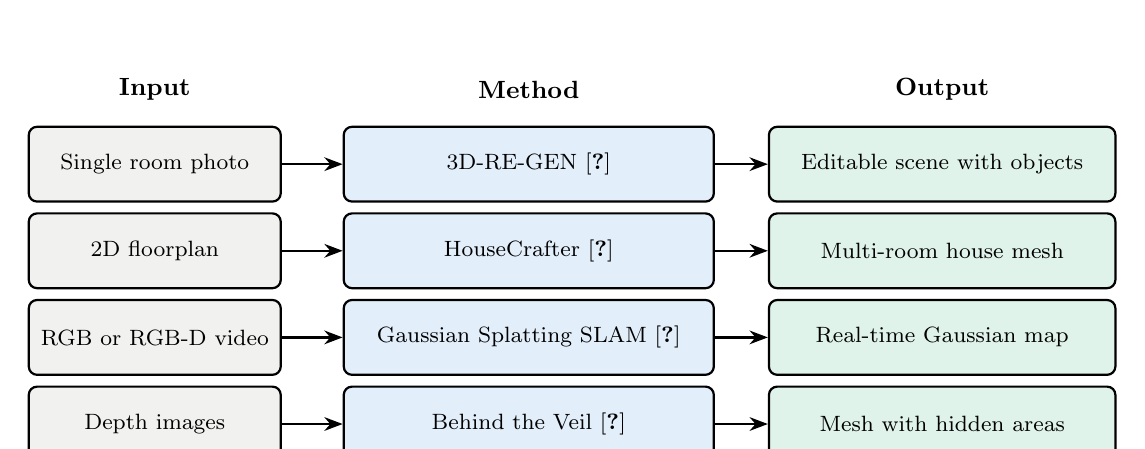
\begin{tikzpicture}[>=Stealth, thick,
  inp/.style={draw, rounded corners=3pt, fill=boxgray, minimum width=3.2cm, minimum height=0.95cm, font=\footnotesize, align=center},
  mth/.style={draw, rounded corners=3pt, fill=boxblue, minimum width=4.7cm, minimum height=0.95cm, font=\footnotesize, align=center},
  outp/.style={draw, rounded corners=3pt, fill=boxgreen, minimum width=4.4cm, minimum height=0.95cm, font=\footnotesize, align=center}]
\foreach \n/\y/\i/\m/\o in {a/3.3/Single room photo/3D-RE-GEN \cite{p1}/Editable scene with objects,b/2.2/2D floorplan/HouseCrafter \cite{p2}/Multi-room house mesh,c/1.1/RGB or RGB-D video/Gaussian Splatting SLAM \cite{p3}/Real-time Gaussian map,d/0/Depth images/Behind the Veil \cite{p4}/Mesh with hidden areas} {
  \node[inp] (i\n) at (0,\y) {\i};
  \node[mth] (m\n) at (4.75,\y) {\m};
  \node[outp] (o\n) at (10.0,\y) {\o};
  \draw[->] (i\n) -- (m\n); \draw[->] (m\n) -- (o\n);
}
\node[font=\small\bfseries] at (0,4.25) {Input};
\node[font=\small\bfseries] at (4.75,4.25) {Method};
\node[font=\small\bfseries] at (10.0,4.25) {Output};
\end{tikzpicture}
\caption{Inputs and outputs of the reviewed indoor 3D methods}
\label{fig:inputs}
\end{figure}

\section{Motivation}

\paragraph{} Three needs motivate this study: \textbf{casual capture}, since homeowners, agents, and designers want 3D rooms from a phone or a floorplan rather than from expensive scanning \cite{p1,p2}; \textbf{editability and completeness}, since virtual staging requires moving or swapping furniture without revealing holes or floating objects \cite{p1,p4}; and \textbf{speed}, since interactive design and AR need models that are built and rendered in real time rather than over hours \cite{p3}.

\section{Problem Statement}

\paragraph{} \emph{Given sparse 2D input about an indoor space---a single photograph, a floorplan, a video, or depth images---produce a photorealistic, geometrically complete, and editable 3D model of the space, efficiently enough to support interactive design, real-estate visualisation, and digital-twin applications.}

\section{Objectives}

\paragraph{} The objectives of this seminar are:
\begin{itemize}
  \item To introduce 3D scene representations, NeRF, 3D Gaussian Splatting, signed distance fields, diffusion models, and visual SLAM.
  \item To review in depth four recent works on single-image reconstruction, floorplan lifting, Gaussian Splatting SLAM, and occluded surface completion.
  \item To compare their inputs, representations, editability, and performance, and to identify open challenges for home and interior design.
\end{itemize}

\section{Scope}

\paragraph{} The seminar covers room- and house-scale indoor scenes, including furniture, walls, and floors, reconstructed or generated from images, floorplans, video, and depth, together with the datasets and metrics used to evaluate them. Outdoor scenes and dynamic humans are outside its scope.

\section{Advantages}

\paragraph{} Neural 3D representations offer several advantages over legacy CAD and photogrammetry workflows:
\begin{itemize}
  \item \textbf{Photorealism:} radiance fields capture reflections, soft lighting, and fine detail.
  \item \textbf{Low Capture Cost:} a phone camera, a single image, or a floorplan can be enough.
  \item \textbf{Completeness:} learned priors fill in regions that were never observed.
  \item \textbf{Interactivity:} Gaussian Splatting renders scenes in real time for walkthroughs and AR.
\end{itemize}

\section{Organization of the Report}

\paragraph{} \textbf{Chapter 2} introduces the theoretical foundations. \textbf{Chapter 3} reviews the four works in detail. \textbf{Chapter 4} compares the approaches, \textbf{Chapter 5} discusses applications, \textbf{Chapter 6} presents challenges and future directions, and \textbf{Chapter 7} concludes the report.

% ================= CHAPTER 2: THEORETICAL FOUNDATIONS =================
\chapter{Theoretical Foundations}

\paragraph{} This chapter introduces the concepts on which the reviewed works build: 3D scene representations, neural radiance fields, 3D Gaussian Splatting, signed distance fields and mesh extraction, diffusion models for 3D content, visual SLAM, and the evaluation metrics used in indoor reconstruction.

\section{3D Scene Representations}

\paragraph{} A 3D scene can be stored \textbf{explicitly}, as point clouds, voxel grids, or triangle meshes, or \textbf{implicitly}, as a function that a neural network evaluates at any 3D point \cite{p4}. Meshes are compact and are what CAD tools, game engines, and physics simulators expect, but fusing new observations into them is difficult. Voxel grids are easy to update but use much memory at fixed resolution. Implicit fields are continuous and can fill small holes, but must be queried point by point. Gaussian splats combine an explicit, flexible set of primitives with smooth, differentiable rendering \cite{p3}. Table~\ref{tab:repr} compares these options.

{\renewcommand{\arraystretch}{1.15}
\begin{table}[htbp]
\centering
\caption{3D scene representations for indoor reconstruction}\label{tab:repr}
\small
\begin{tabularx}{\textwidth}{|>{\raggedright\arraybackslash}p{3.0cm}|X|X|p{1.4cm}|}
\hline
\textbf{Representation} & \textbf{Strength} & \textbf{Weakness} & \textbf{Used in} \\ \hline
Triangle mesh & Editable; standard for CAD, games, physics & Hard to fuse and optimise & \cite{p1,p2,p4} \\ \hline
Voxel grid / TSDF & Simple fusion of depth & Memory-hungry; fixed resolution & \cite{p2} \\ \hline
Neural implicit field & Continuous; fills small holes & Slow per-point queries & \cite{p4} \\ \hline
3D Gaussians & Real-time, differentiable rendering & No explicit surface & \cite{p3} \\ \hline
\end{tabularx}
\end{table}}

\section{Neural Radiance Fields}

\paragraph{} A \textbf{Neural Radiance Field} \cite{mildenhall2020} represents a scene with a multi-layer perceptron (MLP) $F_\Theta$ that maps a 3D position $\mathbf{x}=(x,y,z)$ and viewing direction $(\theta,\phi)$ to a colour $\mathbf{c}$ and a volume density $\sigma$. A pixel is rendered by marching along its camera ray $\mathbf{r}(t)=\mathbf{o}+t\mathbf{d}$ and accumulating colour weighted by density:
\begin{equation}
\hat{C}(\mathbf{r})=\sum_{i=1}^{N}T_i\big(1-e^{-\sigma_i\delta_i}\big)\mathbf{c}_i,\qquad T_i=\exp\Big(-\sum_{j<i}\sigma_j\delta_j\Big),
\end{equation}
where $\delta_i$ is the distance between samples and $T_i$ the transmittance. Because this rendering is differentiable, $F_\Theta$ is trained simply by minimising the difference between rendered and observed pixels across many photographs. NeRF captures view-dependent effects and fine detail, but its per-pixel ray marching makes training and rendering slow \cite{p3}.

\section{3D Gaussian Splatting}

\paragraph{} \textbf{3D Gaussian Splatting} \cite{kerbl2023} replaces the MLP with a large set of anisotropic 3D Gaussians, each with a mean $\boldsymbol{\mu}$, covariance $\Sigma$, colour $c_i$, and opacity $\alpha_i$. To render a view with camera pose $T_{CW}$, each Gaussian is projected to a 2D Gaussian on the image plane,
\begin{equation}
\boldsymbol{\mu}_I=\pi\big(T_{CW}\,\boldsymbol{\mu}_W\big),\qquad \Sigma_I=JW\Sigma_WW^{\top}J^{\top},
\end{equation}
where $\pi$ is the projection, $W$ the rotation of $T_{CW}$, and $J$ the Jacobian of the projection, and the sorted Gaussians are alpha-blended:
\begin{equation}
C_p=\sum_{i\in\mathcal{N}}c_i\,\alpha_i\prod_{j=1}^{i-1}(1-\alpha_j).
\end{equation}
Because it \emph{rasterises} primitives instead of marching rays, 3DGS skips empty space and renders at hundreds of frames per second while remaining fully differentiable \cite{p3}.

\section{Signed Distance Fields and Mesh Extraction}

\paragraph{} A \textbf{signed distance function} (SDF) gives, for every point, its distance to the nearest surface, negative inside objects and positive outside; the surface is its zero level set. Neural SDFs such as DeepSDF \cite{park2019} learn shapes as continuous functions. In \textbf{TSDF fusion} \cite{curless1996}, depth images are integrated into a voxel grid of truncated signed distances by weighted averaging, as in KinectFusion \cite{newcombe2011}. The \textbf{Marching Cubes} algorithm \cite{lorensen1987} then extracts a triangle mesh from the zero crossings of any SDF grid. HouseCrafter fuses its generated RGB-D images with TSDF fusion \cite{p2}, and Behind the Veil predicts SDFs with neural decoders before running Marching Cubes \cite{p4}.

\section{Diffusion Models for 3D Content}

\paragraph{} \textbf{Diffusion models} learn to generate images by reversing a gradual noising process. \textbf{Latent diffusion}, as in Stable Diffusion \cite{rombach2022}, performs this denoising in the compressed latent space of a variational autoencoder (VAE), using a UNet with attention layers that can be conditioned on text, images, or layouts. Because 3D data is scarce while 2D images are abundant, many 3D methods fine-tune such 2D models to produce consistent \emph{multi-view} images, which are then fused into 3D \cite{p2}, or use image-editing and image-to-3D models as components of a larger pipeline \cite{p1}.

\section{Visual SLAM}

\paragraph{} \textbf{Simultaneous Localisation and Mapping} (SLAM) estimates a camera's trajectory while building a map of its surroundings from a video stream. The camera pose at each frame is a rigid transformation $T_{CW}\in SE(3)$, optimised in its Lie algebra so that updates stay valid rotations. \emph{Tracking} estimates the pose of each new frame against the map, and \emph{mapping} refines the map from a window of selected \emph{keyframes}. Monocular SLAM uses a single colour camera and must also infer depth; RGB-D SLAM uses a depth sensor. Map-centric systems maintain one global 3D representation, such as voxels, surfels, or neural fields, and track against it \cite{p3}.

\section{Evaluation Metrics}

\paragraph{} The reviewed works evaluate geometry, appearance, and tracking with different metrics (Table~\ref{tab:metrics}). \textbf{Accuracy} and \textbf{completeness} measure how much of the predicted surface lies near the ground truth and vice versa, and their harmonic mean is the \textbf{F-score}; \textbf{Chamfer} and \textbf{Hausdorff} distances measure average and worst-case point distances \cite{p1,p4}. Rendered images are compared with PSNR, SSIM, and LPIPS \cite{p3}, and generated images are judged with FID and Inception Score \cite{p2}. Camera tracking is measured by the absolute trajectory error (ATE) \cite{p3}.

{\renewcommand{\arraystretch}{1.15}
\begin{table}[htbp]
\centering
\caption{Evaluation metrics used in the reviewed works}\label{tab:metrics}
\small
\begin{tabularx}{\textwidth}{|>{\raggedright\arraybackslash}p{3.4cm}|X|p{1.6cm}|}
\hline
\textbf{Metric} & \textbf{Measures} & \textbf{Used in} \\ \hline
Chamfer, Hausdorff, F-score, IoU & Geometric agreement of scenes and object boxes & \cite{p1} \\ \hline
Accuracy, completeness, F1 & Surface quality, including hidden regions & \cite{p4} \\ \hline
PSNR, SSIM, LPIPS & Quality of rendered views & \cite{p1,p2,p3} \\ \hline
FID, Inception Score & Realism of generated images & \cite{p2} \\ \hline
ATE RMSE & Camera tracking error & \cite{p3} \\ \hline
User studies & Perceived quality and layout & \cite{p1,p2} \\ \hline
\end{tabularx}
\end{table}}

\section{Taxonomy of Approaches}

\paragraph{} Figure~\ref{fig:taxonomy} organises the reviewed works by the task they solve. Two \emph{generate} 3D scenes from limited 2D input---one image \cite{p1} or a floorplan \cite{p2}---and two \emph{reconstruct} scenes from measurements---a live video \cite{p3} or depth images whose hidden regions must be completed \cite{p4}.

\begin{figure}[htbp]
\centering
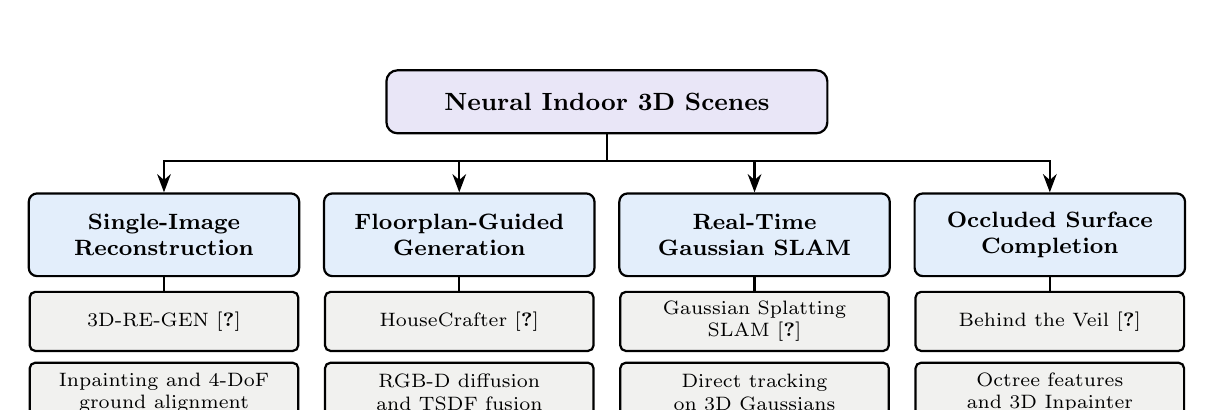
\begin{tikzpicture}[>=Stealth, thick,
  root/.style={draw, rounded corners=4pt, fill=boxviolet, font=\small\bfseries, minimum width=5.6cm, minimum height=0.8cm, align=center},
  cat/.style={draw, rounded corners=3pt, fill=boxblue, font=\footnotesize\bfseries, text width=3.2cm, align=center, minimum height=1.05cm, anchor=north},
  leaf/.style={draw, rounded corners=2pt, fill=boxgray, font=\scriptsize, text width=3.2cm, align=center, minimum height=0.75cm, inner sep=3pt, anchor=north}]
\node[root] (r) at (5.625,0) {Neural Indoor 3D Scenes};
\foreach \x/\n/\t/\la/\lb in {0/a/Single-Image\\ Reconstruction/3D-RE-GEN \cite{p1}/Inpainting and 4-DoF ground alignment,3.75/b/Floorplan-Guided\\ Generation/HouseCrafter \cite{p2}/RGB-D diffusion and TSDF fusion,7.5/c/Real-Time\\ Gaussian SLAM/Gaussian Splatting\\ SLAM \cite{p3}/Direct tracking on 3D Gaussians,11.25/d/Occluded Surface\\ Completion/Behind the Veil \cite{p4}/Octree features and 3D Inpainter} {
  \node[cat] (\n) at (\x,-1.15) {\t};
  \draw[->] (r.south) -- (5.625,-0.75) -| (\n.north);
  \node[leaf] (\n1) at (\x,-2.4) {\la};
  \node[leaf] at (\x,-3.3) {\lb};
  \draw (\n.south) -- (\n1.north);
}
\end{tikzpicture}
\caption{Taxonomy of the reviewed approaches}
\label{fig:taxonomy}
\end{figure}

% ================= CHAPTER 3: LITERATURE SURVEY =================
\chapter{Literature Survey}

\paragraph{} This chapter reviews the four works in detail. For each, it describes the problem and motivation, the method, the experimental setup and results, and closes with a short discussion of strengths and limitations.

% ---------------------------------------------------------------
\section{3D-RE-GEN: 3D Reconstruction of Indoor Scenes with a Generative Framework}

\paragraph{} The base paper, by Sautter, Dihlmann, and Lensch \cite{p1}, from the University of T\"ubingen, presents \textbf{3D-RE-GEN}, a compositional framework that turns a single photograph of a room into a textured background mesh and a set of separate, textured 3D objects that can be moved, relit, and simulated (Figure~\ref{fig:p1_teaser}).

\begin{figure}[htbp]
\centering
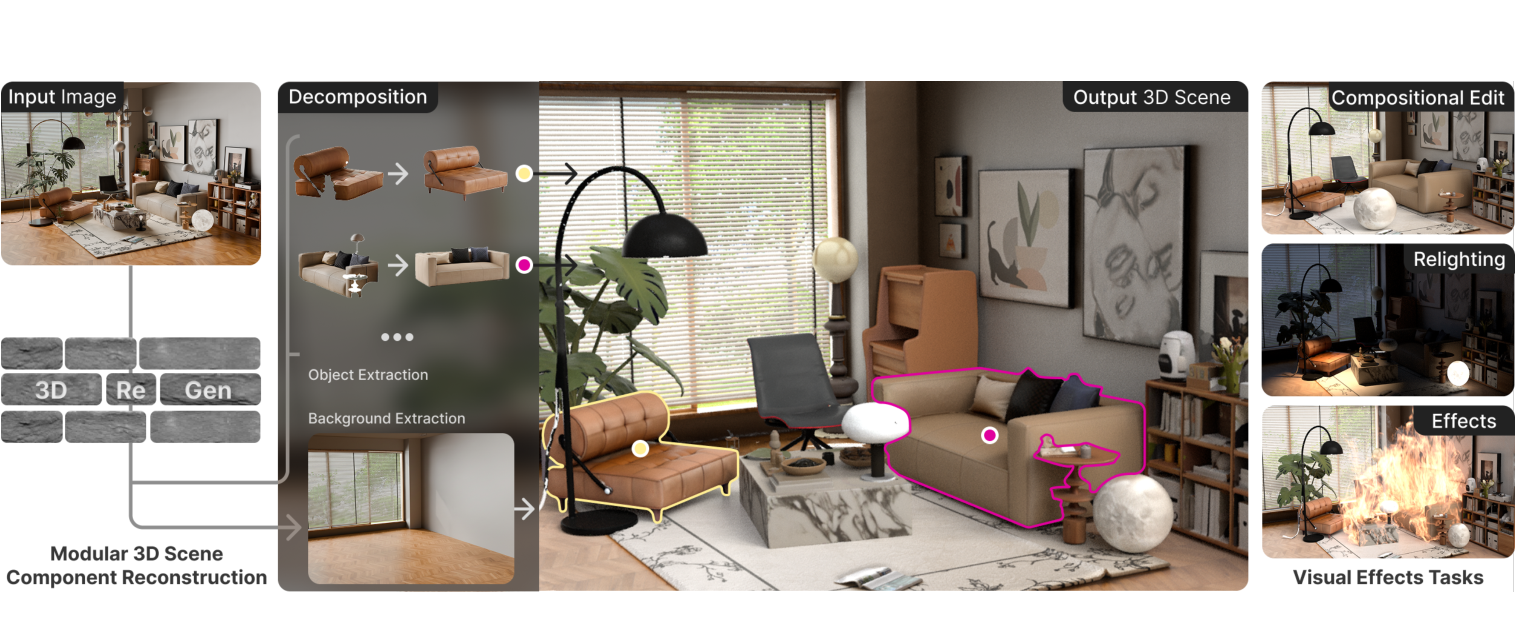
\includegraphics[width=\textwidth]{figs/p1_teaser.png}
\caption[3D-RE-GEN decomposes a single image into an editable scene]{3D-RE-GEN decomposes a single image into an editable scene \cite{p1}}
\label{fig:p1_teaser}
\end{figure}

\subsection{Problem Statement and Motivation}

\paragraph{} Building a 3D interior by hand is a production bottleneck: the room, every piece of furniture, and the final layout are each modelled by specialised artists. Single-image-to-3D models such as SF3D and Hunyuan3D work well for isolated objects but fail on cluttered multi-object scenes, where the image lacks depth, objects hide one another, and nothing states their distances, scale, or contact points \cite{p1}. Earlier holistic, retrieval-based, and compositional methods share two gaps: the \emph{background} of walls and floor is usually ignored, and nothing enforces \emph{physical plausibility}, so objects float above or sink into the floor.

\subsection{Method}

\paragraph{} 3D-RE-GEN chains strong pretrained models and adds two novel contributions, namely \textbf{Application-Querying} for occluded objects and a \textbf{4-DoF ground-constrained optimisation} for layout (Figure~\ref{fig:p1_framework}).

\begin{figure}[htbp]
\centering
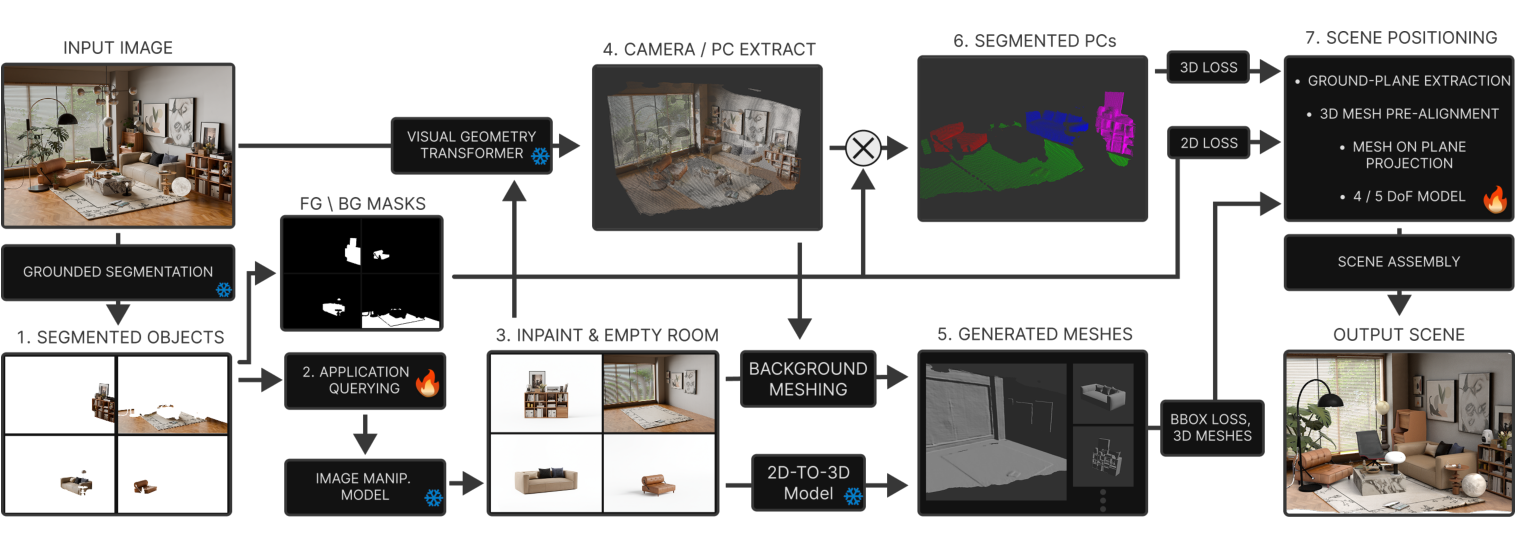
\includegraphics[width=\textwidth]{figs/p1_framework.png}
\caption[Overview of the 3D-RE-GEN framework]{Overview of the 3D-RE-GEN framework \cite{p1}}
\label{fig:p1_framework}
\end{figure}

\paragraph{} \textbf{Segmentation.} Grounded SAM performs text-prompted instance segmentation of the input image $I$, and a lightweight tool lets the user correct the masks $M_{obj}$, which later serve as 2D silhouette targets \cite{p1}.

\paragraph{} \textbf{Application-Querying (A-Q).} Asking a generative model to complete a partially hidden object often fails because it lacks scene context. A-Q builds a composite query image styled like a user interface with two panels: the full image with the target outlined, and the occluded segment on a white background. An image-editing model (Gemini 2.5 Flash Image) is asked to return the same interface with the object completed, so it infers hidden parts with consistent perspective, lighting, and material (Figure~\ref{fig:p1_aq}). The same model removes all objects to produce an ``empty room'' image $I_{bg}$ \cite{p1}.

\begin{figure}[htbp]
\centering
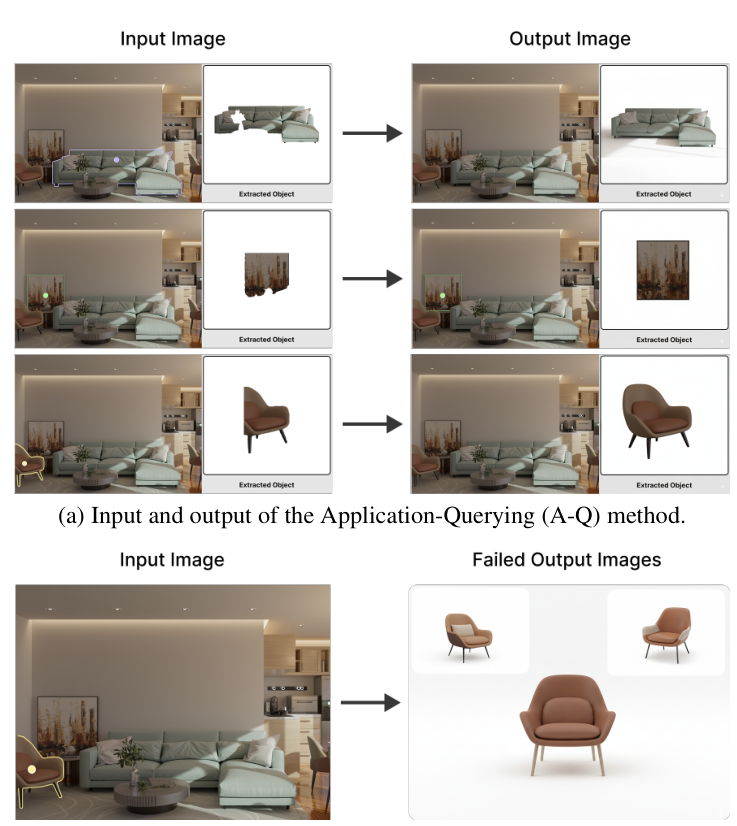
\includegraphics[width=0.5\textwidth]{figs/p1_aq.png}
\caption[Application-Querying with a GUI-style visual prompt]{Application-Querying with a GUI-style visual prompt \cite{p1}}
\label{fig:p1_aq}
\end{figure}

\paragraph{} \textbf{Scene, camera, and assets.} The geometry transformer VGGT receives both $I$ and $I_{bg}$ and returns aligned cameras and point clouds; the background cloud is meshed into a background usable for rendering and simulation, and back-projected masks cut per-object target clouds $P_{target}$ from the scene cloud. Each completed object image is converted into a textured mesh by Hunyuan3D 2.0 \cite{p1}.

\paragraph{} \textbf{Differentiable placement.} Objects whose masks touch the floor mask use the \textbf{4-DoF planar model}; others use a 5-DoF model (translation, yaw, scale). The floor plane is fitted with RANSAC, and in its local frame the planar model learns only a 2D translation $(t'_x,t'_z)$, a yaw $r'_y$, and a scale $s$:
\begin{equation}
V_{world}=T_{plane\rightarrow world}\big(s\,R_y(r'_y)\,V_{local}+(t'_x,\,0,\,t'_z)^{\top}\big),
\end{equation}
so objects can only slide and rotate on the floor. Both models minimise
\begin{equation}
\mathcal{L}_{total}=w_{sil}\,\mathcal{L}_{silhouette}+w_{3D}\,\mathcal{L}_{3D}+w_{bbox}\,\mathcal{L}_{bbox},
\end{equation}
combining a Dice and Focal silhouette loss, a point-to-face distance to $P_{target}$, and a penalty on vertices that leave the background bounding box \cite{p1}.

\subsection{Experimental Setup}

\paragraph{} The training-free pipeline uses PyTorch3D for differentiable rendering; a room with about ten objects takes 17--20 minutes on one GPU, or 7--8 minutes on four. Evaluation uses hand-picked synthetic CGTrader scenes, unseen by competing methods trained on 3D-FRONT, plus real photographs. Scenes are normalised and aligned with ICP, then compared with Chamfer distance, F-score, bounding-box IoU, and Hausdorff distance against MIDI and DepR \cite{p1}.

\subsection{Results and Analysis}

\paragraph{} As Table~\ref{tab:p1_main} shows, 3D-RE-GEN outperforms both baselines on every metric: its Chamfer distance of 0.011 is less than a third of MIDI's, its F-score reaches 0.85, its IoU of 0.63 shows correct relative object placement, and its Hausdorff distance of 0.33 indicates few outliers or floating artefacts. MIDI often merges or duplicates objects and DepR produces misaligned ``blobs''. In a study with 59 participants, 3D-RE-GEN received 81\% of the preferences, mostly for its layout \cite{p1}.

{\renewcommand{\arraystretch}{1.12}
\begin{table}[htbp]
\centering
\caption{3D-RE-GEN against MIDI and DepR}\label{tab:p1_main}
\small
\begin{tabular}{|l|c|c|c|c|c|c|}
\hline
\textbf{Method} & \textbf{CD $\downarrow$} & \textbf{F-Score $\uparrow$} & \textbf{IoU $\uparrow$} & \textbf{Precision $\uparrow$} & \textbf{Recall $\uparrow$} & \textbf{Hausdorff $\downarrow$} \\ \hline
DepR & 0.028 & 0.65 & 0.44 & 0.12 & 0.18 & 0.61 \\ \hline
MIDI & 0.036 & 0.70 & 0.57 & 0.15 & 0.13 & 0.55 \\ \hline
3D-RE-GEN & \textbf{0.011} & \textbf{0.85} & \textbf{0.63} & \textbf{0.21} & \textbf{0.19} & \textbf{0.33} \\ \hline
\end{tabular}
\end{table}}

\paragraph{} \textbf{Ablation.} Without the 4-DoF model, objects drift off the floor and Chamfer distance rises to 0.019; without A-Q, the 3D generator sees only occluded segments and the F-score drops to 0.68, with sharply worse perceptual scores (Table~\ref{tab:p1_ablation}) \cite{p1}.

{\renewcommand{\arraystretch}{1.12}
\begin{table}[htbp]
\centering
\caption{Ablation of the 4-DoF model and Application-Querying}\label{tab:p1_ablation}
\small
\begin{tabular}{|l|c|c|c|c|c|c|}
\hline
\textbf{Variant} & \textbf{CD $\downarrow$} & \textbf{F-Score $\uparrow$} & \textbf{IoU $\uparrow$} & \textbf{Hausdorff $\downarrow$} & \textbf{SSIM $\uparrow$} & \textbf{LPIPS $\downarrow$} \\ \hline
Without 4-DoF & 0.019 & 0.82 & 0.52 & 0.51 & 0.27 & 0.46 \\ \hline
Without A-Q & 0.030 & 0.68 & 0.51 & 0.52 & 0.13 & 0.66 \\ \hline
Full 3D-RE-GEN & \textbf{0.011} & \textbf{0.85} & \textbf{0.63} & \textbf{0.33} & \textbf{0.29} & \textbf{0.43} \\ \hline
\end{tabular}
\end{table}}

\subsection{Discussion}

\paragraph{} 3D-RE-GEN outputs exactly what designers need---separate textured furniture on a complete background---and is training-free and modular. Its limitations are its dependence on several large, partly proprietary models, minutes of runtime per room, occasional manual mask correction, a small evaluation set, and a ground-plane assumption that does not cover wall-mounted or stacked objects.

% ---------------------------------------------------------------
\section{HouseCrafter: Lifting Floorplans to 3D Scenes with 2D Diffusion Models}

\paragraph{} Chen, Nguyen, Voleti, Jampani, and Jiang \cite{p2}, from Northeastern University and Stability AI, present \textbf{HouseCrafter}, which turns a 2D floorplan---walls, doors, windows, and furniture boxes---into a complete, textured 3D house mesh using a pretrained image diffusion model (Figure~\ref{fig:p2_overview}).

\begin{figure}[htbp]
\centering
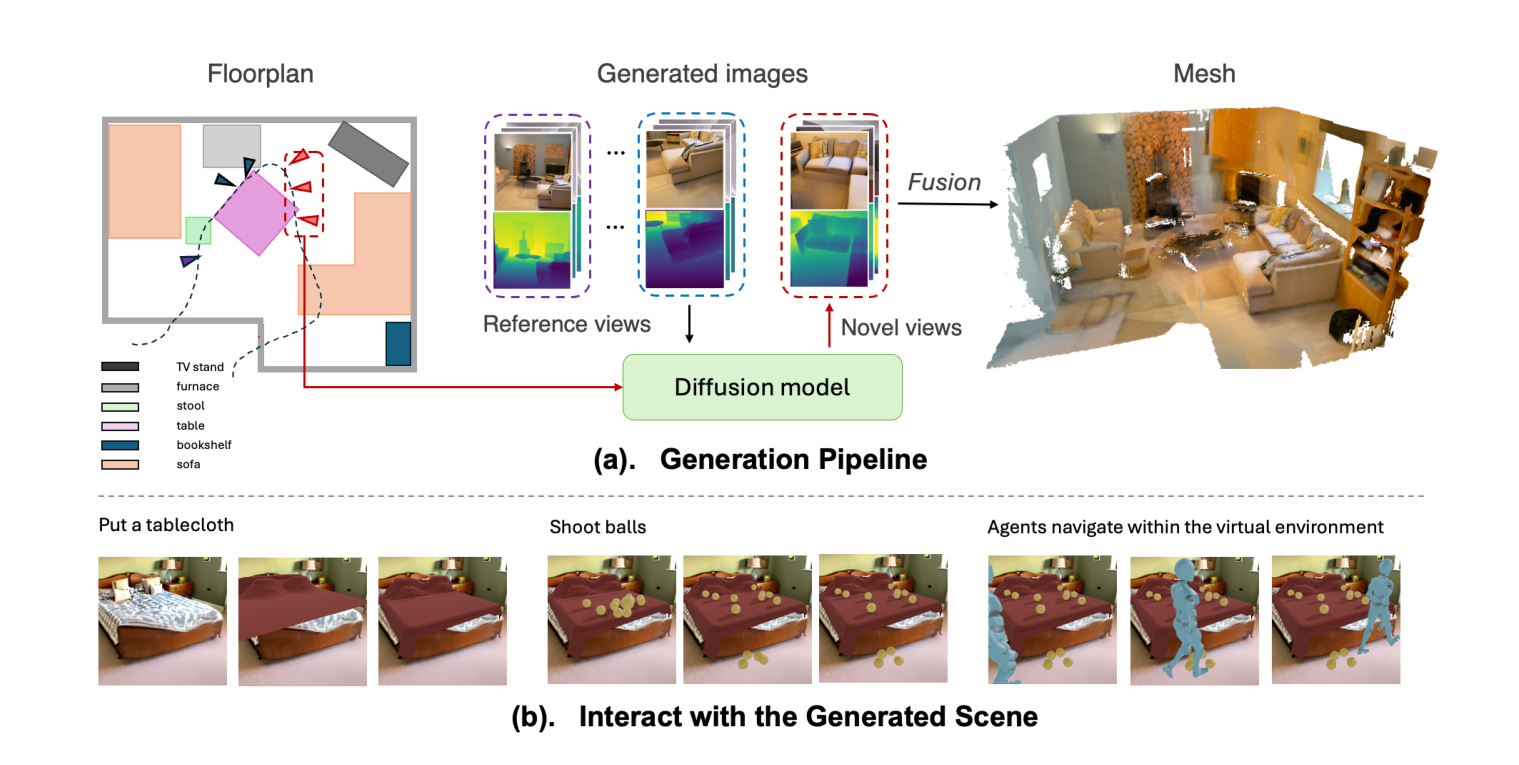
\includegraphics[width=0.86\textwidth]{figs/p2_overview.png}
\caption[HouseCrafter generation pipeline and scene interaction]{HouseCrafter generation pipeline and scene interaction \cite{p2}}
\label{fig:p2_overview}
\end{figure}

\subsection{Problem Statement and Motivation}

\paragraph{} 3D data is scarce compared with web-scale images, so training 3D generators directly is hard. Multi-view diffusion models work for single objects, whose views fit in one batch, but not for houses. Text-guided methods such as Text2Room build rooms image by image with monocular depth, suffering scale ambiguity and lacking global structure, and 3D proxy boxes become cumbersome for large scenes. A 2D floorplan is a familiar, intuitive way to specify a whole house \cite{p2}.

\subsection{Method}

\paragraph{} \textbf{Autoregressive generation.} Camera locations sampled over the free space of the floorplan form a graph that is traversed batch by batch: images already generated at visited nodes within $r$ hops serve as references for novel views at unvisited nodes within $n$ hops, and the first batch is conditioned on the floorplan alone. TSDF fusion finally integrates all RGB-D images into a mesh \cite{p2}.

\paragraph{} \textbf{Joint RGB-D diffusion.} The UNet of Stable Diffusion v1.5 \cite{rombach2022} is fine-tuned with its VAE frozen (Figure~\ref{fig:p2_model}). RGB and depth latents are concatenated, $z=[x,d]$, and denoised jointly; depth is clipped to 0--3 metres and replicated to three channels for the VAE. Generating \emph{metric} depth avoids the scale ambiguity of monocular estimators \cite{p2}.

\begin{figure}[htbp]
\centering
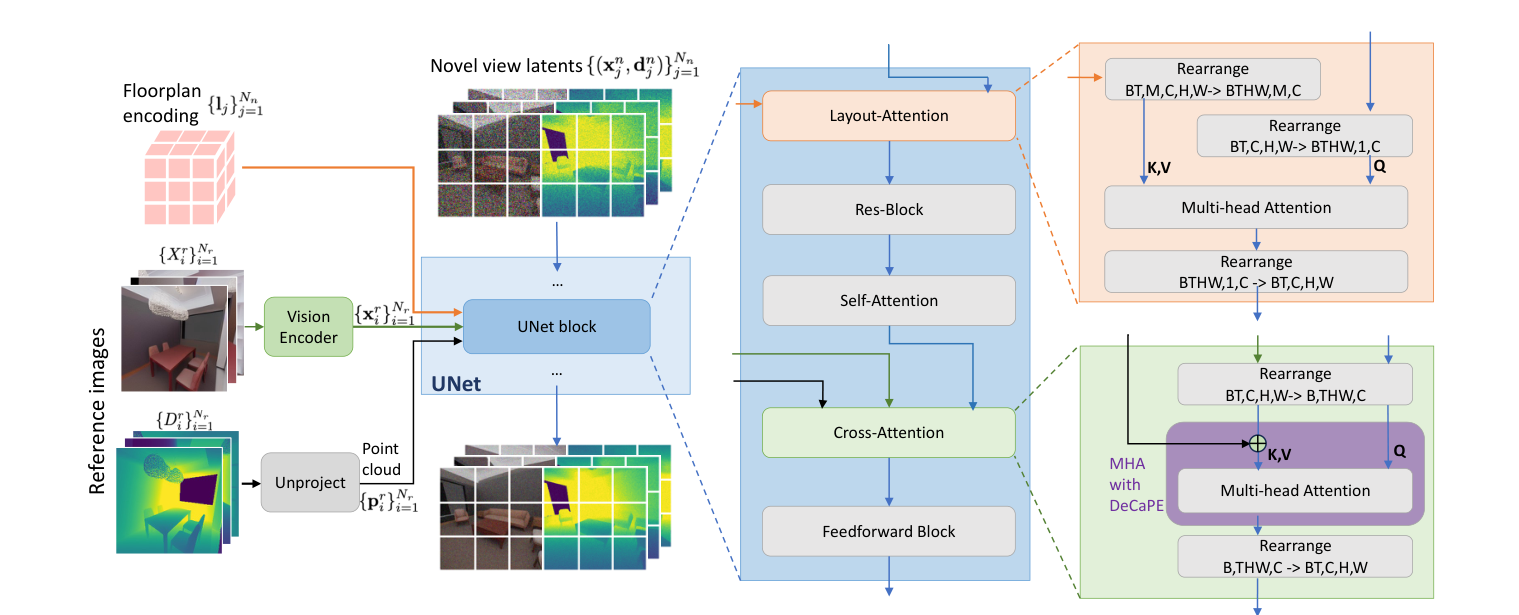
\includegraphics[width=\textwidth]{figs/p2_model.png}
\caption[Floorplan-guided RGB-D generation model]{Floorplan-guided RGB-D generation model \cite{p2}}
\label{fig:p2_model}
\end{figure}

\paragraph{} \textbf{Floorplan conditioning.} For every latent pixel, the camera ray is projected onto the floor plane and up to $M$ intersections with floorplan components are collected, stopping at the first wall. Each intersection's category $c$ and position $p$ are embedded as $l=\mathrm{Embed}(c)+\mathrm{PosEnc}(p)$, and a \textbf{layout-attention} layer at the start of each UNet block lets every pixel attend to the floorplan along its own ray \cite{p2}.

\paragraph{} \textbf{Depth-enhanced camera encoding.} Novel views attend to reference views through cross-attention. Extending camera positional encoding (CaPE), \textbf{DeCaPE} adds the 3D position $p_K$ of each reference token, obtained from its depth:
\begin{equation}
s_{QK}=v_Q^{\top}\,\phi\big(\pi_Q^{-1}\pi_K\big)\big(v_K+\mathrm{PosEnc}(p_K)\big),
\end{equation}
which depends only on relative poses and makes attention geometry-aware \cite{p2}.

\subsection{Experimental Setup}

\paragraph{} About 2{,}000 3D-FRONT houses with 2 million renders are used for training and 300 for evaluation. Metrics are FID and Inception Score; PSNR and depth error between reference and novel (R-N) and between novel (N-N) views; floorplan consistency, measured by segmenting the scene with ODIN and computing mAP@25 against the floorplan boxes; and the number of dangling components. Baselines are CC3D, BlockFusion with Meshy textures, and Text2Room, and a 12-person user study is added \cite{p2}.

\subsection{Results and Analysis}

\paragraph{} HouseCrafter achieves the highest floorplan consistency (Table~\ref{tab:p2_main}), with mAP@25 of 45.77 against 25.60 for CC3D, approaching 54.51 for ground-truth images. Text2Room and BlockFusion score higher Inception Scores, which the authors attribute to models trained on real images; even ground-truth renders score only 4.50. Users strongly preferred HouseCrafter for quality and floorplan consistency \cite{p2}.

{\renewcommand{\arraystretch}{1.12}
\begin{table}[htbp]
\centering
\caption{HouseCrafter against scene generation baselines}\label{tab:p2_main}
\small
\begin{tabular}{|l|c|c|c|}
\hline
\textbf{Method} & \textbf{IS $\uparrow$} & \textbf{mAP@25 $\uparrow$} & \textbf{Artifacts $\downarrow$} \\ \hline
Text2Room & \textbf{5.35} & -- & 302.5 \\ \hline
CC3D & 4.02 & 25.60 & -- \\ \hline
BlockFusion + Meshy & 5.01 & 0.81 & \textbf{118.64} \\ \hline
HouseCrafter & 4.37 & \textbf{45.77} & 178.0 \\ \hline
Ground-truth images & 4.50 & 54.51 & -- \\ \hline
\end{tabular}
\end{table}}

\paragraph{} \textbf{Ablation.} Generating depth with RGB lowers FID from 49.35 to 33.39; floorplan conditioning is the largest gain, cutting FID to about 16 and N-N depth error below 8; and DeCaPE gives the lowest depth errors and raises mAP@25 to 52.26 (Table~\ref{tab:p2_ablation}) \cite{p2}.

{\renewcommand{\arraystretch}{1.12}
\begin{table}[htbp]
\centering
\caption{Ablation of HouseCrafter design choices}\label{tab:p2_ablation}
\small
\setlength{\tabcolsep}{5pt}
\begin{tabular}{|l|c|c|c|c|c|}
\hline
\multirow{2}{*}{\textbf{Variant}} & \textbf{FID $\downarrow$} & \textbf{PSNR $\uparrow$} & \textbf{AbsRel $\downarrow$} & \textbf{AbsRel $\downarrow$} & \textbf{mAP@25 $\uparrow$} \\
 & & \textbf{R-N} & \textbf{R-N} & \textbf{N-N} & \\ \hline
RGB only & 49.35 & -- & -- & -- & -- \\ \hline
+ Output depth & 33.39 & 20.99 & 23.56 & 11.48 & -- \\ \hline
+ Input depth & 35.77 & 20.91 & 22.28 & 12.05 & -- \\ \hline
+ Floorplan (no input depth) & \textbf{15.64} & \textbf{25.36} & 7.65 & 7.85 & 48.46 \\ \hline
+ Floorplan and input depth & 16.70 & 24.47 & 7.73 & 8.20 & 49.74 \\ \hline
+ DeCaPE (full) & 17.75 & 25.31 & \textbf{6.79} & \textbf{7.37} & \textbf{52.26} \\ \hline
\end{tabular}
\end{table}}

\subsection{Discussion}

\paragraph{} HouseCrafter's strength is its interface: a floorplan, which architects and agents already have, controls a whole house, and the output is an explicit mesh. Reusing an image diffusion model avoids large 3D training sets. Its limitations are training on synthetic houses, a coarse vertex-coloured mesh not separated into objects, many diffusion steps per house, and floorplans that specify footprints but not style or height.

% ---------------------------------------------------------------
\section{Gaussian Splatting SLAM}

\paragraph{} Matsuki, Murai, Kelly, and Davison \cite{p3}, from Imperial College London, present the first SLAM system that uses \textbf{3D Gaussian Splatting} as its only scene representation. From a single moving camera it tracks the camera pose and builds a photorealistic Gaussian map live at about 3 frames per second, capturing thin wires and even transparent glass, and it extends naturally to RGB-D input.

\subsection{Problem Statement and Motivation}

\paragraph{} Every dense SLAM map has a weakness: voxel grids are memory-hungry with bounded resolution, meshes need irregular topology updates, surfels are hard to optimise, and neural fields need expensive per-pixel ray casting. 3DGS \cite{kerbl2023} is as flexible as a point cloud yet continuous and differentiable, rendering up to 200 frames per second at 1080p, but it had been used only offline, with camera poses computed beforehand by structure from motion. A live system must estimate poses and grow the map simultaneously \cite{p3}.

\subsection{Method}

\paragraph{} Tracking, keyframing, and mapping share one Gaussian map (Figure~\ref{fig:p3_system}). Colour is alpha-blended as in Chapter~2, and depth likewise, $D_p=\sum_{i}z_i\,\alpha_i\prod_{j<i}(1-\alpha_j)$ \cite{p3}.

\begin{figure}[htbp]
\centering
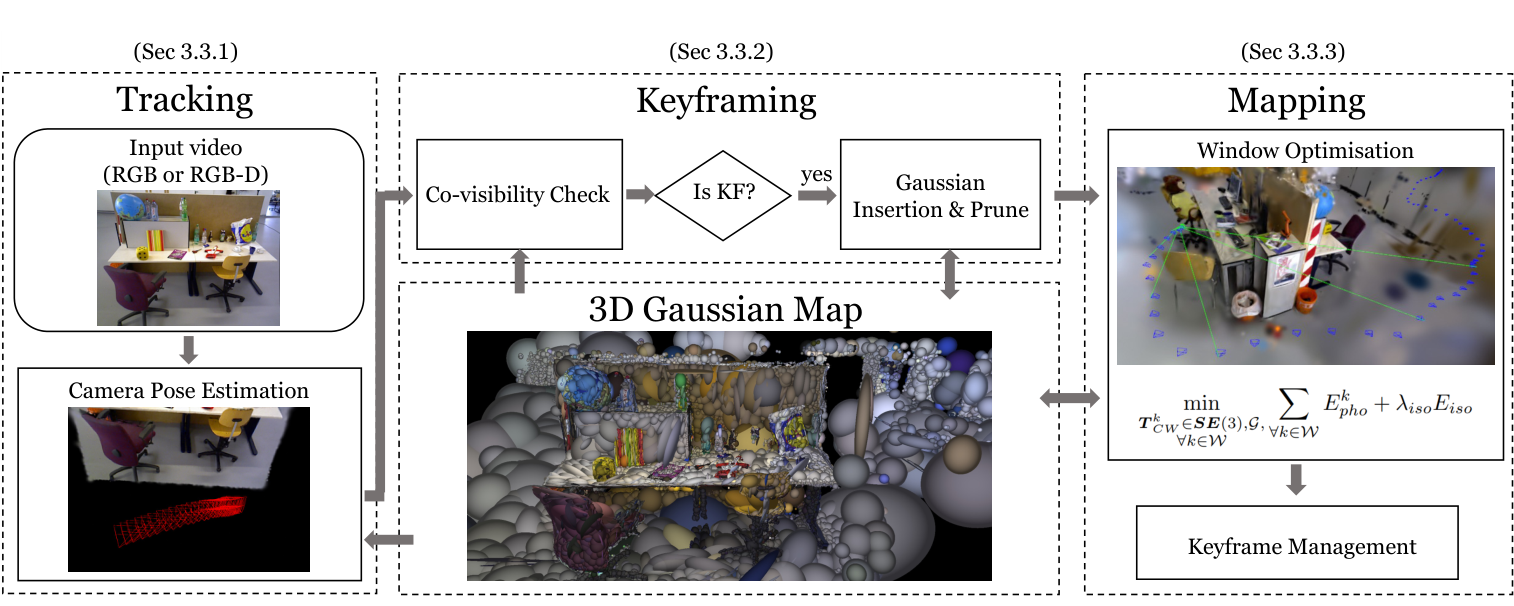
\includegraphics[width=\textwidth]{figs/p3_system.png}
\caption[Overview of the Gaussian Splatting SLAM system]{Overview of the Gaussian Splatting SLAM system \cite{p3}}
\label{fig:p3_system}
\end{figure}

\paragraph{} \textbf{Tracking.} For every new frame only the camera pose $T_{CW}$ is optimised, with the map fixed, by minimising the photometric residual
\begin{equation}
E_{pho}=\big\|I(\mathcal{G},T_{CW})-\bar{I}\big\|_1,
\end{equation}
plus a depth residual $E_{geo}=\|D(\mathcal{G},T_{CW})-\bar{D}\|_1$ when depth is available. As tracking needs at least 50 iterations per frame, the authors derive the first analytic Jacobians of projected Gaussians with respect to the pose on the Lie group $SE(3)$, for example
\begin{equation}
\frac{D\boldsymbol{\mu}_C}{DT_{CW}}=\begin{bmatrix}\mathbf{I} & -\boldsymbol{\mu}_C^{\times}\end{bmatrix},
\end{equation}
where $^{\times}$ is the skew-symmetric matrix, implemented in CUDA inside the rasteriser \cite{p3}.

\paragraph{} \textbf{Keyframing.} A small keyframe window $\mathcal{W}_k$ is optimised. A Gaussian is visible in a view if it is rasterised before the accumulated opacity reaches 0.5, so occlusion is handled naturally; a frame becomes a keyframe when the IoU of its visible Gaussians with the last keyframe drops below a threshold. New Gaussians are inserted at keyframes from measured or rendered depth, and recent Gaussians not seen by at least three other frames are pruned \cite{p3}.

\paragraph{} \textbf{Mapping.} Mapping refines the Gaussians and keyframe poses in the window plus two random past keyframes. Because rasterisation does not constrain a Gaussian's extent along the viewing ray, Gaussians tend to become long needles that create artefacts and disturb tracking, so an \textbf{isotropic regularisation} penalises each Gaussian's scales $\mathbf{s}_i$ for differing from their mean $\tilde{s}_i$:
\begin{equation}
E_{iso}=\sum_{i=1}^{|\mathcal{G}|}\big\|\mathbf{s}_i-\tilde{s}_i\mathbf{1}\big\|_1,\qquad \min_{T^{k}_{CW},\,\mathcal{G}}\;\sum_{k\in\mathcal{W}}E^{k}_{pho}+\lambda_{iso}E_{iso},
\end{equation}
with geometric residuals added when depth is available \cite{p3}.

\subsection{Experimental Setup}

\paragraph{} Evaluation uses three real TUM RGB-D sequences (monocular and RGB-D), eight synthetic Replica sequences (RGB-D), and live RealSense D455 captures, on an Intel i9-12900K with an RTX 4090. Tracking is measured by ATE RMSE and maps by PSNR, SSIM, and LPIPS on non-keyframes, averaged over three runs. Baselines without loop closure are DSO, DROID-VO, and DepthCov-VO for monocular input, and neural-field SLAM systems such as NICE-SLAM, ESLAM, Co-SLAM, and Point-SLAM for RGB-D input \cite{p3}.

\subsection{Results and Analysis}

\paragraph{} \textbf{Tracking.} On TUM (Table~\ref{tab:p3_tum}), with a single camera and no learned depth prior, the method averages 3.96 cm against 7.73 cm for DROID-VO; with RGB-D input it averages 1.47 cm, the best among compared methods and close to ORB-SLAM2 with loop closure (Figure~\ref{fig:p3_ate}). On Replica, its single-process version averages 0.32 cm \cite{p3}.

{\renewcommand{\arraystretch}{1.12}
\begin{table}[htbp]
\centering
\caption{Camera tracking error on the TUM RGB-D dataset}\label{tab:p3_tum}
\small
\begin{tabular}{|l|l|c|c|c|c|}
\hline
\textbf{Input} & \textbf{Method} & \textbf{fr1/desk} & \textbf{fr2/xyz} & \textbf{fr3/office} & \textbf{Avg. (cm)} \\ \hline
\multirow{4}{*}{Monocular} & DSO & 22.4 & \textbf{1.10} & 9.50 & 11.0 \\ \cline{2-6}
 & DROID-VO & 5.20 & 10.7 & 7.30 & 7.73 \\ \cline{2-6}
 & DepthCov-VO & 5.60 & 1.20 & 68.8 & 25.2 \\ \cline{2-6}
 & Gaussian Splatting SLAM & \textbf{3.78} & 4.60 & \textbf{3.50} & \textbf{3.96} \\ \hline
\multirow{4}{*}{RGB-D} & NICE-SLAM & 4.26 & 6.19 & 3.87 & 4.77 \\ \cline{2-6}
 & ESLAM & 2.47 & \textbf{1.11} & 2.42 & 2.00 \\ \cline{2-6}
 & Point-SLAM & 4.34 & 1.31 & 3.48 & 3.04 \\ \cline{2-6}
 & Gaussian Splatting SLAM & \textbf{1.50} & 1.44 & \textbf{1.49} & \textbf{1.47} \\ \hline
\end{tabular}
\end{table}}

\begin{figure}[htbp]
\centering
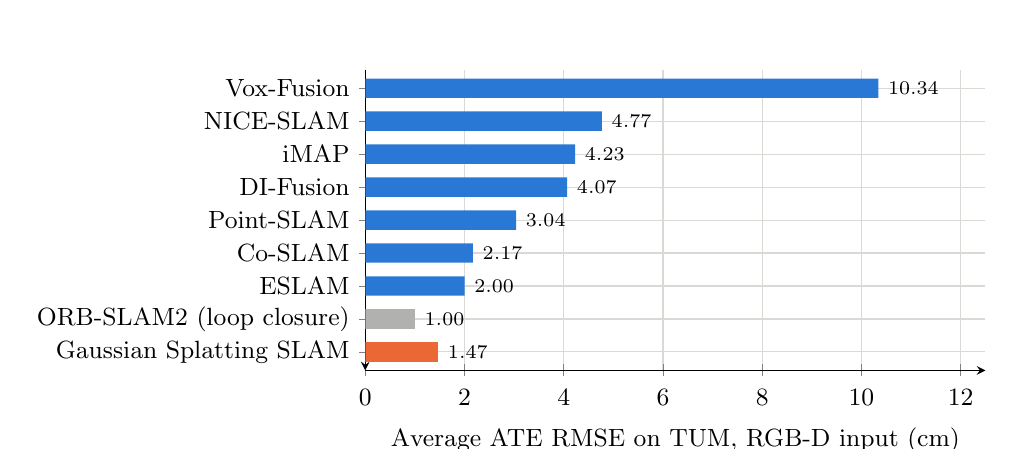
\begin{tikzpicture}
\begin{axis}[xbar, width=0.78\textwidth, height=5.4cm, bar width=7pt, xmin=0, xmax=12.5,
  xlabel={Average ATE RMSE on TUM, RGB-D input (cm)}, symbolic y coords={a,b,c,d,e,f,g,h,i},
  ytick={a,b,c,d,e,f,g,h,i}, yticklabels={Vox-Fusion,NICE-SLAM,iMAP,DI-Fusion,Point-SLAM,Co-SLAM,ESLAM,ORB-SLAM2 (loop closure),Gaussian Splatting SLAM},
  y dir=reverse, axis lines=left, grid=major, grid style={gridgray}, enlarge y limits=0.07,
  nodes near coords, nodes near coords align={horizontal}, every node near coord/.append style={font=\scriptsize, anchor=west},
  point meta=rawx, nodes near coords={\pgfmathprintnumber[fixed, fixed zerofill, precision=2]{\pgfplotspointmeta}}, tick label style={font=\small}, label style={font=\small}]
\addplot[fill=seriesA, draw=none, bar shift=0pt] coordinates {(10.34,a) (4.77,b) (4.23,c) (4.07,d) (3.04,e) (2.17,f) (2.00,g)};
\addplot[fill=inkgray!45, draw=none, bar shift=0pt] coordinates {(1.00,h)};
\addplot[fill=seriesB, draw=none, bar shift=0pt] coordinates {(1.47,i)};
\end{axis}
\end{tikzpicture}
\caption[Average tracking error of RGB-D SLAM methods]{Average tracking error of RGB-D SLAM methods (data from \cite{p3})}
\label{fig:p3_ate}
\end{figure}

\paragraph{} \textbf{Rendering and memory.} On Replica (Table~\ref{tab:p3_render}) the method reaches 38.94 dB PSNR and the lowest LPIPS while rendering at 769 frames per second, hundreds of times faster than neural-field systems; Point-SLAM's slightly higher SSIM relies on ground-truth depth. The map needs only 2.6 MB for monocular and 3.97 MB for RGB-D input on TUM, against 6.4 MB for Co-SLAM \cite{p3}.

{\renewcommand{\arraystretch}{1.12}
\begin{table}[htbp]
\centering
\caption{Novel view rendering on the Replica dataset}\label{tab:p3_render}
\small
\begin{tabular}{|l|c|c|c|c|}
\hline
\textbf{Method} & \textbf{PSNR (dB) $\uparrow$} & \textbf{SSIM $\uparrow$} & \textbf{LPIPS $\downarrow$} & \textbf{Rendering FPS $\uparrow$} \\ \hline
NICE-SLAM & 24.42 & 0.809 & 0.233 & 0.54 \\ \hline
Vox-Fusion & 24.41 & 0.801 & 0.236 & 2.17 \\ \hline
Point-SLAM & 35.17 & \textbf{0.975} & 0.124 & 1.33 \\ \hline
Gaussian Splatting SLAM & \textbf{38.94} & 0.968 & \textbf{0.070} & \textbf{769} \\ \hline
\end{tabular}
\end{table}}

\paragraph{} \textbf{Ablation and convergence.} Removing isotropic regularisation raises monocular ATE from 3.96 to 4.83 cm, and removing keyframe selection raises it to 8.73 cm. Cameras placed up to 1.2 m from a target converge on a Gaussian map in about 80\% of trials, against 33\% for an MLP SDF and 14\% for a hash-grid SDF \cite{p3}.

\subsection{Discussion}

\paragraph{} Gaussian Splatting SLAM shows that a photorealistic model of a room can be built \emph{while} walking through it with an ordinary camera and viewed in real time, with one compact representation for tracking, mapping, and rendering. Its limitations are the lack of loop closure for large homes, about 3 frames per second on a high-end GPU in monocular mode, no clean surface mesh or object separation, and empty regions wherever the camera did not look.

% ---------------------------------------------------------------
\section{Behind the Veil: Enhanced Indoor 3D Scene Reconstruction with Occluded Surfaces Completion}

\paragraph{} Sun, Zhao, Guo, Wang, Huang, Chen, and Ren \cite{p4}, from Purdue University and Bosch Research North America, present a reconstruction method that, from a sequence of depth images, recovers not only the visible surfaces of a room but also the surfaces hidden by occlusion---the back of a sofa, the floor under a bed, and the wall behind a television.

\subsection{Problem Statement and Motivation}

\paragraph{} Virtual touring and room rearrangement need re-configurable scenes: when a sofa is moved, its back and the floor beneath it must not appear as holes. TSDF fusion \cite{curless1996} and surfels are limited by depth noise and blocked views, neural implicit methods such as BNV-Fusion fill only small gaps, and object-centric priors need category-specific pretraining that cannot cover every object in a room \cite{p4}.

\subsection{Method}

\paragraph{} \textbf{Coarse-fine octree.} The unprojected depth points are stored in an $L$-level octree with learnable features at node corners, interpolated trilinearly (Figure~\ref{fig:p4_octree}). With $j=4$ and $L=9$, the levels split into \emph{coarse} features $O_c=\{O_i\}_{i=0}^{j}$, encoding contextual structure that generalises to unseen regions, and \emph{fine} features $O_f=\{O_i\}_{i=j+1}^{L}$, encoding detailed visible geometry \cite{p4}.

\begin{figure}[htbp]
\centering
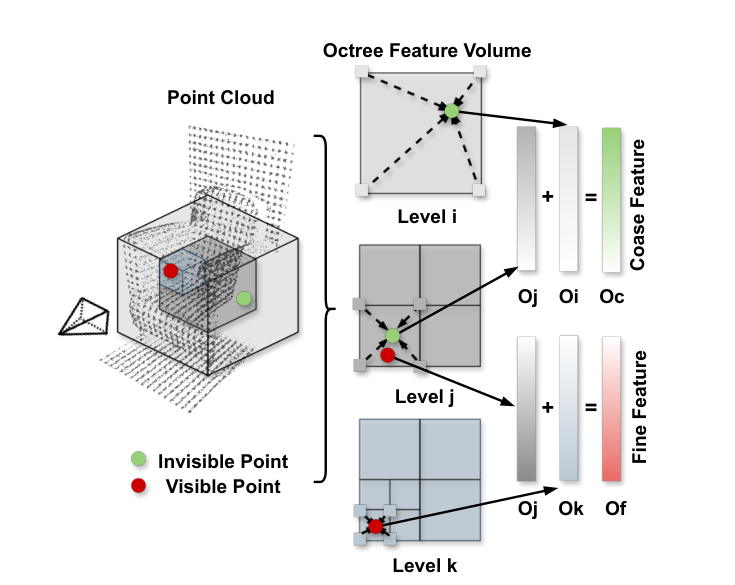
\includegraphics[width=0.42\textwidth]{figs/p4_octree.png}
\caption[Coarse-fine hierarchical octree feature volume]{Coarse-fine hierarchical octree feature volume \cite{p4}}
\label{fig:p4_octree}
\end{figure}

\paragraph{} \textbf{Dual decoders.} Two decoders predict signed distances: a scene-specific \textbf{Geo-decoder} $D_{Geo}$, fed with fine features, for visible surfaces, and a cross-scene \textbf{3D Inpainter} $D_{Ip}$, fed with coarse features, for occluded surfaces. With $f$ a positional encoding,
\begin{equation}
d_{p_v}=D_{Geo}\big(f(p_v),O_f(p_v)\big),\qquad d_{p_i}=D_{Ip}\big(f(p_i),O_c(p_i)\big).
\end{equation}
The method runs in three stages (Figure~\ref{fig:p4_pipeline}) \cite{p4}.

\begin{figure}[htbp]
\centering
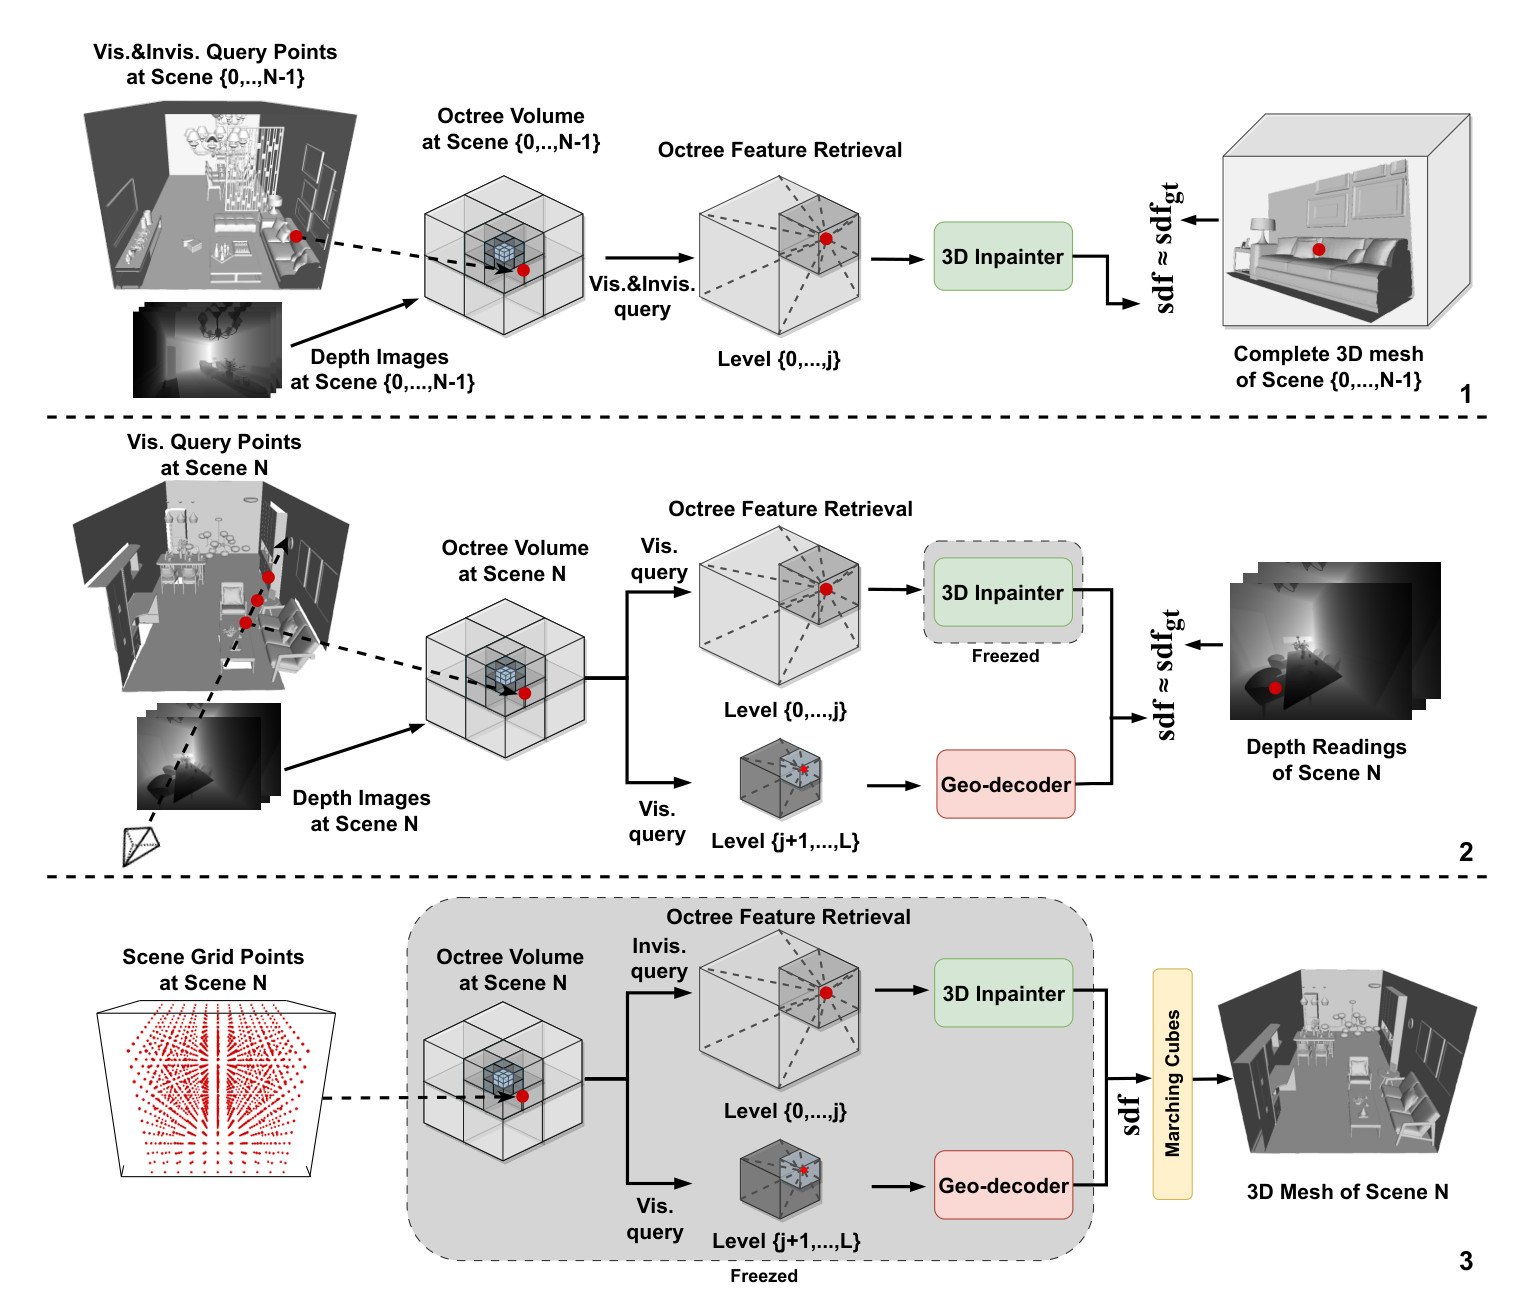
\includegraphics[width=0.64\textwidth]{figs/p4_pipeline.png}
\caption[Three-stage pipeline of Behind the Veil]{Three-stage pipeline of Behind the Veil \cite{p4}}
\label{fig:p4_pipeline}
\end{figure}

\paragraph{} \textbf{Stage 1: training the 3D Inpainter.} Points with ground-truth signed distances are sampled from complete training meshes. In a decoder-only latent-optimisation design, each scene keeps its own octree features while all share the Inpainter, trained with a binary cross-entropy on sigmoid-mapped SDFs plus eikonal and smoothness terms \cite{p4}:
\begin{equation}
\mathcal{L}=\mathcal{L}_{bce}+\lambda_{eik}\big(1-\|\nabla D_{Ip}\|\big)^2+\lambda_{smooth}\big\|\nabla D_{Ip}(p)-\nabla D_{Ip}(p+\epsilon)\big\|^2.
\end{equation}

\paragraph{} \textbf{Stage 2: fitting a new scene.} With only depth images available, points sampled along camera rays near observed surfaces supervise the Geo-decoder and both feature sets, while the Inpainter stays frozen, so the coarse features adapt until the Inpainter explains the visible surfaces and continues them into hidden regions \cite{p4}.

\paragraph{} \textbf{Stage 3: mesh extraction.} Grid points lacking features at more than $\alpha=3$ octree levels are treated as invisible and sent to the Inpainter, the rest to the Geo-decoder, and Marching Cubes \cite{lorensen1987} extracts the complete mesh \cite{p4}.

\subsection{Experimental Setup}

\paragraph{} The authors build the \textbf{3D Completed Room Scene} (3D-CRS) dataset of 20 rooms with complete meshes (15 for training, 5 for testing) and also use iTHOR scenes (6 test scenes) and ScanNet for qualitative tests. Accuracy, completeness, and F1 are compared with TSDF Fusion, Go-Surf, and BNV-Fusion \cite{p4}.

\subsection{Results and Analysis}

\paragraph{} Completeness rises from 76.5 for BNV-Fusion to 89.3 on 3D-CRS and from 72.3 to 89.8 on iTHOR, giving the best F1 on every test scene (Table~\ref{tab:p4_main}). Accuracy is slightly below BNV-Fusion's because it also covers the harder inpainted regions. Baselines leave holes behind sofas and under furniture, whereas Behind the Veil completes planar areas and thin structures alike, leaving a complete room layout after furniture removal (Figure~\ref{fig:p4_layout}) \cite{p4}.

{\renewcommand{\arraystretch}{1.12}
\begin{table}[htbp]
\centering
\caption{Average reconstruction quality on 3D-CRS and iTHOR}\label{tab:p4_main}
\small
\begin{tabular}{|l|c|c|c|c|c|c|}
\hline
\multirow{2}{*}{\textbf{Method}} & \multicolumn{3}{c|}{\textbf{3D-CRS}} & \multicolumn{3}{c|}{\textbf{iTHOR}} \\ \cline{2-7}
 & \textbf{Accu.} & \textbf{Comp.} & \textbf{F1} & \textbf{Accu.} & \textbf{Comp.} & \textbf{F1} \\ \hline
TSDF Fusion & 84.6 & 60.2 & 70.2 & 81.3 & 66.1 & 72.9 \\ \hline
Go-Surf & 90.1 & 70.8 & 79.3 & 88.9 & 69.8 & 78.2 \\ \hline
BNV-Fusion & \textbf{92.5} & 76.5 & 83.7 & \textbf{91.3} & 72.3 & 80.7 \\ \hline
Behind the Veil & 90.4 & \textbf{89.3} & \textbf{89.9} & 88.8 & \textbf{89.8} & \textbf{89.3} \\ \hline
\end{tabular}
\end{table}}

\begin{figure}[htbp]
\centering
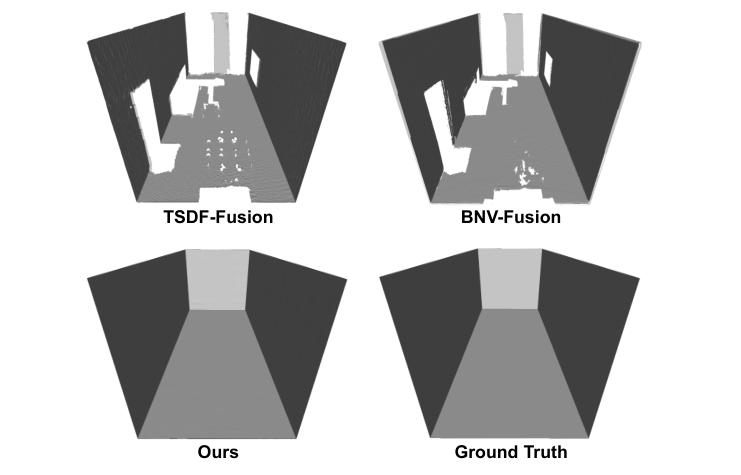
\includegraphics[width=0.5\textwidth]{figs/p4_layout.png}
\caption[Room layout after furniture removal]{Room layout after furniture removal \cite{p4}}
\label{fig:p4_layout}
\end{figure}

\paragraph{} \textbf{Fewer depth frames.} With only 50 depth frames per scene, BNV-Fusion's completeness falls from 76.5 to 62.3, whereas Behind the Veil stays above 87.5 because its Inpainter fills what the frames miss (Figure~\ref{fig:p4_frames}) \cite{p4}.

\begin{figure}[htbp]
\centering
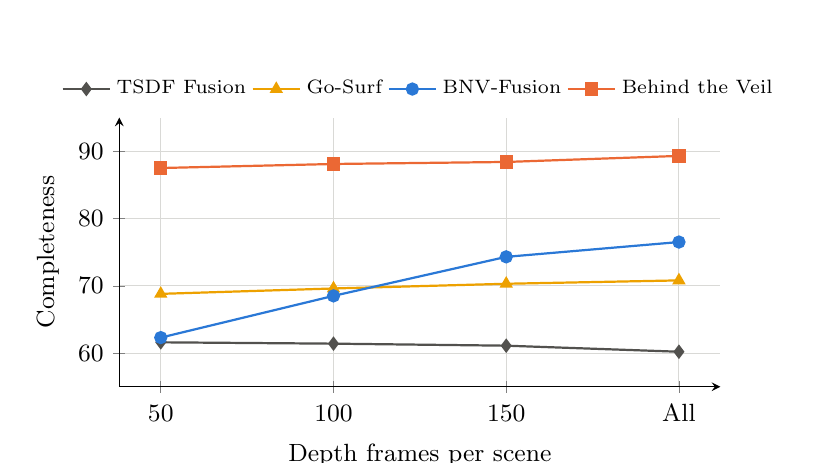
\begin{tikzpicture}
\begin{axis}[width=0.76\textwidth, height=5cm, symbolic x coords={f50,f100,f150,fall}, xtick=data,
  xticklabels={50,100,150,All}, xlabel={Depth frames per scene}, ylabel={Completeness}, ymin=55, ymax=95,
  grid=major, grid style={gridgray}, axis lines=left, enlarge x limits=0.08,
  legend style={at={(0.5,1.03)}, anchor=south, legend columns=4, font=\scriptsize, draw=none},
  tick label style={font=\small}, label style={font=\small}]
\addplot[inkgray, thick, mark=diamond*] coordinates {(f50,61.6) (f100,61.4) (f150,61.1) (fall,60.2)};
\addplot[seriesD, thick, mark=triangle*] coordinates {(f50,68.8) (f100,69.6) (f150,70.3) (fall,70.8)};
\addplot[seriesA, thick, mark=*] coordinates {(f50,62.3) (f100,68.5) (f150,74.3) (fall,76.5)};
\addplot[seriesB, thick, mark=square*] coordinates {(f50,87.5) (f100,88.1) (f150,88.4) (fall,89.3)};
\legend{TSDF Fusion, Go-Surf, BNV-Fusion, Behind the Veil}
\end{axis}
\end{tikzpicture}
\caption[Completeness versus number of depth frames]{Completeness versus number of depth frames (data from \cite{p4})}
\label{fig:p4_frames}
\end{figure}

\paragraph{} \textbf{Ablation.} Without a cross-scene Inpainter, completeness stays near BNV-Fusion's level; coarse features alone lose accuracy and fine features alone lose completeness (Table~\ref{tab:p4_ablation}) \cite{p4}.

{\renewcommand{\arraystretch}{1.12}
\begin{table}[htbp]
\centering
\caption{Ablation of the 3D Inpainter and coarse-fine features}\label{tab:p4_ablation}
\small
\begin{tabular}{|l|c|c|c|}
\hline
\textbf{Variant} & \textbf{Accu.} & \textbf{Comp.} & \textbf{F1} \\ \hline
Without 3D Inpainter & \textbf{91.4} & 82.2 & 86.5 \\ \hline
Without cross-scene training & 83.3 & 82.4 & 82.9 \\ \hline
Only coarse features & 86.0 & 88.5 & 87.2 \\ \hline
Only fine features & 86.6 & 82.2 & 84.3 \\ \hline
Full method & 89.1 & \textbf{90.1} & \textbf{89.7} \\ \hline
\end{tabular}
\end{table}}

\subsection{Discussion}

\paragraph{} Behind the Veil solves a problem central to virtual staging: once furniture moves, the surfaces behind and beneath it must exist. Its split between a scene-specific decoder and a shared Inpainter, trained on only 15 rooms, generalises even to real ScanNet data. Its limitations are geometry without colour, the need for posed depth images, completed surfaces that are plausible guesses, and per-scene optimisation that is not real-time.

% ---------------------------------------------------------------
\section{Summary of the Literature Survey}

\paragraph{} Table~\ref{tab:survey} summarises the four reviewed works.

{\renewcommand{\arraystretch}{1.15}
\begin{table}[htbp]
\centering
\caption{Summary of the reviewed works}\label{tab:survey}
\small
\begin{tabularx}{\textwidth}{|p{2.3cm}|p{1.6cm}|>{\raggedright\arraybackslash}p{2.2cm}|X|>{\raggedright\arraybackslash}p{2.6cm}|}
\hline
\textbf{Work} & \textbf{Venue} & \textbf{Input} & \textbf{Key idea} & \textbf{Output} \\ \hline
3D-RE-GEN \cite{p1} & arXiv 2025 & One RGB image & Application-Querying inpainting and 4-DoF ground-aligned placement of generated assets & Textured objects on a background mesh \\ \hline
HouseCrafter \cite{p2} & ICCV 2025 & 2D floorplan & Floorplan-guided multi-view RGB-D diffusion with DeCaPE, fused by TSDF & Multi-room house mesh \\ \hline
Gaussian Splatting SLAM \cite{p3} & CVPR 2024 & RGB or RGB-D video & Analytic $SE(3)$ Jacobians, isotropic regularisation, and Gaussian keyframing & Live 3D Gaussian map and camera path \\ \hline
Behind the Veil \cite{p4} & CVPR 2025 & Depth images with poses & Coarse-fine octree with Geo-decoder and cross-scene 3D Inpainter & Complete mesh including hidden surfaces \\ \hline
\end{tabularx}
\end{table}}

% ================= CHAPTER 4: DISCUSSION AND COMPARISON =================
\chapter{Discussion and Comparison}

\paragraph{} This chapter compares the four works along the dimensions that matter for home and interior design: what input they need, how they represent the scene, how editable and complete the result is, how fast they run, and how they are evaluated.

\section{Comparison of Methodologies}

\paragraph{} Table~\ref{tab:method_cmp} compares the methods. Two are \emph{generative}---they invent content the input does not show, using large pretrained models---and two are \emph{reconstructive}---they recover measured geometry and appearance, adding only learned priors where measurements are missing.

{\renewcommand{\arraystretch}{1.15}
\begin{table}[htbp]
\centering
\caption{Comparison of the reviewed methodologies}\label{tab:method_cmp}
\small
\begin{tabularx}{\textwidth}{|p{2.6cm}|X|X|X|X|}
\hline
\textbf{Aspect} & \textbf{3D-RE-GEN} & \textbf{HouseCrafter} & \textbf{GS SLAM} & \textbf{Behind the Veil} \\ \hline
Paradigm & Generative, compositional & Generative, autoregressive & Reconstructive, online & Reconstructive with completion \\ \hline
Representation & Textured meshes & RGB-D views fused to TSDF mesh & 3D Gaussians & Octree features and SDF \\ \hline
Learned prior & Pretrained detection, editing, and 3D models & Fine-tuned Stable Diffusion & None & Inpainter trained on complete rooms \\ \hline
Training needed & None & Large synthetic house set & None & Small set of complete rooms \\ \hline
Separate objects & Yes & No & No & No \\ \hline
Colour or texture & Yes & Yes & Yes & No \\ \hline
Speed & Minutes per scene & Many diffusion steps & Live & Per-scene optimisation \\ \hline
\end{tabularx}
\end{table}}

\section{Input Requirements and Representations}

\paragraph{} The methods form a spectrum of input effort. 3D-RE-GEN needs only one photograph, and HouseCrafter only a floorplan, so both suit early design stages when no scan exists. Gaussian Splatting SLAM needs a walkthrough video, and Behind the Veil needs posed depth images, so both suit capturing an existing home. Less input means more of the output is \emph{imagined}: a single image cannot show the back of a wardrobe, and a floorplan says nothing about upholstery, so the generative methods trade fidelity to the real space for convenience \cite{p1,p2}. Representations follow from the goal: meshes for editing and export (3D-RE-GEN, HouseCrafter), Gaussians for fast, photorealistic viewing (Gaussian Splatting SLAM), and neural SDFs for clean, complete geometry (Behind the Veil) \cite{p3,p4}.

\section{Editability and Completeness}

\paragraph{} Virtual staging requires two properties: objects that can be moved independently, and surfaces that remain complete after they move. Only 3D-RE-GEN produces separate object meshes, and its 4-DoF placement keeps them on the floor \cite{p1}. HouseCrafter's fused house is one mesh, although the floorplan itself can be edited and the house regenerated \cite{p2}. Gaussian Splatting SLAM's map is easy to modify locally because Gaussians are independent primitives, but it has no object structure \cite{p3}. Behind the Veil is the only method that explicitly fills in surfaces hidden behind and under furniture, which is exactly what is revealed when an object is moved \cite{p4}. The works are therefore complementary: object decomposition from \cite{p1} combined with occluded-surface completion from \cite{p4} would yield fully editable rooms.

\section{Real-Time Versus Offline Operation}

\paragraph{} Gaussian Splatting SLAM is the only live system, mapping at about 3 frames per second and rendering at hundreds, which suits AR previews and walkthroughs \cite{p3}. 3D-RE-GEN takes 7--20 minutes per room, HouseCrafter runs many diffusion batches, and Behind the Veil optimises per scene \cite{p1,p2,p4}; this suits one-off model creation, but interactive editing needs faster, feed-forward variants. Because each work uses different data and metrics, their numbers cannot be compared directly, and generative methods also rely on user studies \cite{p1,p2}.

\section{Strengths and Limitations}

\paragraph{} Table~\ref{tab:strength_limit} summarises the main strengths and limitations identified in Chapter~3.

{\renewcommand{\arraystretch}{1.15}
\begin{table}[htbp]
\centering
\caption{Strengths and limitations of the reviewed works}\label{tab:strength_limit}
\small
\begin{tabularx}{\textwidth}{|p{2.5cm}|X|X|}
\hline
\textbf{Work} & \textbf{Strengths} & \textbf{Limitations} \\ \hline
3D-RE-GEN & Separate textured objects and background; no training; objects grounded on the floor & Minutes per scene; relies on large proprietary models; hidden parts are imagined \\ \hline
HouseCrafter & Whole houses from a familiar floorplan; metric depth; explicit mesh & Trained on synthetic houses; single fused mesh; floorplan omits style and height \\ \hline
Gaussian Splatting SLAM & Live tracking and photorealistic mapping; compact; real-time rendering & No loop closure; no surface mesh or objects; unseen areas stay empty \\ \hline
Behind the Veil & Completes hidden surfaces; generalises from few rooms; clean meshes & Geometry only; needs posed depth; not real-time \\ \hline
\end{tabularx}
\end{table}}

\section{Towards a Combined Home Design Workflow}

\paragraph{} Figure~\ref{fig:workflow} sketches how the four methods could form one pipeline. A floorplan is lifted into an initial house model \cite{p2}; once the home exists, a walkthrough video produces a live photorealistic map \cite{p3}, and its depth is completed behind and beneath furniture \cite{p4}; finally, individual pieces captured in photographs are turned into separate, ground-aligned assets that designers can move, replace, and restyle \cite{p1}.

\begin{figure}[htbp]
\centering
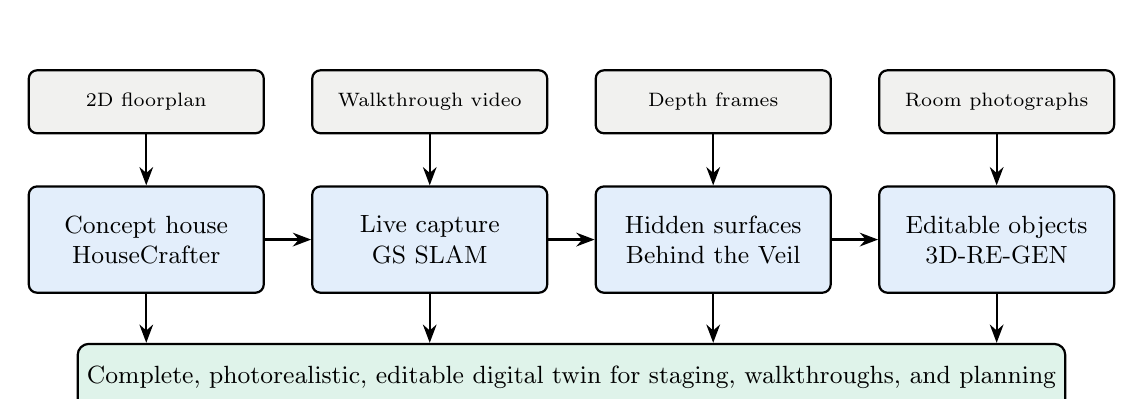
\begin{tikzpicture}[>=Stealth, thick,
  stage/.style={draw, rounded corners=3pt, fill=boxblue, text width=2.75cm, minimum height=1.35cm, align=center, font=\small},
  io/.style={draw, rounded corners=3pt, fill=boxgray, text width=2.75cm, minimum height=0.8cm, align=center, font=\scriptsize}]
\node[io] (i1) at (0,1.75) {2D floorplan};
\node[io] (i2) at (3.6,1.75) {Walkthrough video};
\node[io] (i3) at (7.2,1.75) {Depth frames};
\node[io] (i4) at (10.8,1.75) {Room photographs};
\node[stage] (s1) at (0,0) {Concept house\\ HouseCrafter};
\node[stage] (s2) at (3.6,0) {Live capture\\ GS SLAM};
\node[stage] (s3) at (7.2,0) {Hidden surfaces\\ Behind the Veil};
\node[stage] (s4) at (10.8,0) {Editable objects\\ 3D-RE-GEN};
\foreach \a/\b in {i1/s1,i2/s2,i3/s3,i4/s4} \draw[->] (\a) -- (\b);
\foreach \a/\b in {s1/s2,s2/s3,s3/s4} \draw[->] (\a) -- (\b);
\node[draw, rounded corners=4pt, fill=boxgreen, minimum width=12.4cm, minimum height=0.85cm, font=\small, align=center] (out) at (5.4,-1.75) {Complete, photorealistic, editable digital twin for staging, walkthroughs, and planning};
\foreach \s in {s1,s2,s3,s4} \draw[->] (\s) -- (\s |- out.north);
\end{tikzpicture}
\caption{A combined home design workflow}
\label{fig:workflow}
\end{figure}

% ================= CHAPTER 5: APPLICATIONS =================
\chapter{Applications}

\paragraph{} Neural 3D scene representations open many applications in the home and interior sector.

\section{Virtual Staging and Interior Design}

\paragraph{} Designers can turn a client's photograph into an editable 3D room, remove or replace furniture, and render the result from new viewpoints \cite{p1}. Completed occluded surfaces mean that floors and walls stay intact when pieces are moved \cite{p4}, and ground-aligned placement keeps new items physically plausible.

\section{Real Estate Walkthroughs}

\paragraph{} Agents can capture a property with a phone and publish a photorealistic, real-time walkthrough built by Gaussian Splatting SLAM \cite{p3}, while developers can present unbuilt apartments as complete 3D houses generated from their floorplans \cite{p2}.

\section{Architectural Digital Twins and Home Automation}

\paragraph{} Complete, accurate room models form digital twins for facility management, renovation planning, and smart homes, where devices and sensors are placed in a 3D model of the space. Complete geometry also lets home robots, such as cleaners, plan around and beneath furniture \cite{p4}.

\section{AR, VR, and E-Commerce}

\paragraph{} Furniture retailers can let customers place products in a 3D model of their own room in AR, and VR users can explore generated homes and interact with them, for example by placing a tablecloth or letting virtual agents navigate inside \cite{p2}.

% ================= CHAPTER 6: CHALLENGES AND FUTURE DIRECTIONS =================
\chapter{Challenges and Future Directions}

\section{Open Challenges}

\begin{itemize}
  \item \textbf{Fidelity versus imagination:} generative methods invent hidden content that may not match the real home, which matters for measurements and purchases \cite{p1,p2}.
  \item \textbf{Speed:} most methods take minutes or longer per room; only SLAM runs live, and only on a high-end GPU \cite{p3}.
  \item \textbf{Semantics and editability:} few outputs separate objects, materials, and lighting, which design tools need \cite{p1}.
  \item \textbf{Scale and drift:} whole homes need loop closure and consistent multi-room models \cite{p2,p3}.
  \item \textbf{Data and evaluation:} complete real indoor scenes with ground truth are rare, and generative quality lacks reliable metrics \cite{p2,p4}.
\end{itemize}

\section{Future Directions}

\begin{itemize}
  \item \textbf{Unified pipelines} that combine live Gaussian capture with object decomposition and occluded-surface completion.
  \item \textbf{Feed-forward models} that reconstruct or generate a room in seconds rather than minutes.
  \item \textbf{Material and lighting decomposition}, so that staged rooms can be relit and refurnished realistically.
  \item \textbf{Language and layout control}, letting users restyle rooms by text while respecting floorplans.
  \item \textbf{On-device capture} on phones and AR headsets for consumer use.
\end{itemize}

% ================= CHAPTER 7: CONCLUSION =================
\chapter{Conclusion}

\paragraph{} This seminar examined how Neural Radiance Fields and related neural 3D representations, especially 3D Gaussian Splatting, are transforming the creation of indoor 3D environments for home and interior design. After introducing scene representations, volume rendering, Gaussian splatting, signed distance fields, diffusion models, and visual SLAM, it reviewed four recent works in depth.

\paragraph{} \textbf{3D-RE-GEN} reconstructs an editable room with separate, ground-aligned furniture and a complete background from a single image, using Application-Querying and a 4-DoF planar optimisation \cite{p1}. \textbf{HouseCrafter} lifts a 2D floorplan into a multi-room house by generating consistent RGB-D views with a floorplan-guided diffusion model and fusing them into a mesh \cite{p2}. \textbf{Gaussian Splatting SLAM} builds a photorealistic Gaussian map live from a single camera with analytic pose Jacobians and isotropic regularisation \cite{p3}. \textbf{Behind the Veil} completes the surfaces hidden behind and beneath furniture with a coarse-fine octree and a cross-scene 3D Inpainter \cite{p4}.

\paragraph{} Together, these works show that the bottlenecks of legacy CAD modelling and photogrammetry---manual effort, expensive capture, incomplete and non-editable meshes---can be overcome by learned 3D priors. They are complementary: generative methods minimise input, reconstructive methods ensure fidelity, and their combination points towards complete, photorealistic, and editable digital twins of homes. Faster and unified pipelines that also model materials and lighting will make such tools practical for everyday virtual staging, real-estate walkthroughs, and automated spatial design.

% ================= REFERENCES =================
\begingroup
\setstretch{1.15}
\begin{thebibliography}{99}
\addcontentsline{toc}{chapter}{References}

\bibitem{p1}
T. Sautter, J.-N. Dihlmann, and H. Lensch, ``3D-RE-GEN: 3D reconstruction of indoor scenes with a generative framework,'' arXiv preprint arXiv:2512.17459, 2025.

\bibitem{p2}
Y. Chen, H. T. Nguyen, V. Voleti, V. Jampani, and H. Jiang, ``HouseCrafter: Lifting floorplans to 3D scenes with 2D diffusion models,'' in \textit{Proc. IEEE/CVF ICCV}, 2025, pp. 28440--28449.

\bibitem{p3}
H. Matsuki, R. Murai, P. H. J. Kelly, and A. J. Davison, ``Gaussian splatting SLAM,'' in \textit{Proc. IEEE/CVF CVPR}, 2024, pp. 18039--18048.

\bibitem{p4}
S. Sun, C. Zhao, Y. Guo, \textit{et al.}, ``Behind the veil: Enhanced indoor 3D scene reconstruction with occluded surfaces completion,'' in \textit{Proc. IEEE/CVF CVPR}, 2025, pp. 12744--12753.

\bibitem{mildenhall2020}
B. Mildenhall, P. P. Srinivasan, M. Tancik, \textit{et al.}, ``NeRF: Representing scenes as neural radiance fields for view synthesis,'' in \textit{Proc. ECCV}, 2020, pp. 405--421.

\bibitem{kerbl2023}
B. Kerbl, G. Kopanas, T. Leimk\"uhler, and G. Drettakis, ``3D Gaussian splatting for real-time radiance field rendering,'' \textit{ACM Trans. Graphics}, vol. 42, no. 4, 2023.

\bibitem{rombach2022}
R. Rombach, A. Blattmann, D. Lorenz, P. Esser, and B. Ommer, ``High-resolution image synthesis with latent diffusion models,'' in \textit{Proc. IEEE/CVF CVPR}, 2022, pp. 10684--10695.

\bibitem{park2019}
J. J. Park, P. Florence, J. Straub, \textit{et al.}, ``DeepSDF: Learning continuous signed distance functions for shape representation,'' in \textit{Proc. IEEE/CVF CVPR}, 2019, pp. 165--174.

\bibitem{curless1996}
B. Curless and M. Levoy, ``A volumetric method for building complex models from range images,'' in \textit{Proc. ACM SIGGRAPH}, 1996, pp. 303--312.

\bibitem{newcombe2011}
R. A. Newcombe, S. Izadi, O. Hilliges, \textit{et al.}, ``KinectFusion: Real-time dense surface mapping and tracking,'' in \textit{Proc. IEEE ISMAR}, 2011, pp. 127--136.

\bibitem{lorensen1987}
W. E. Lorensen and H. E. Cline, ``Marching cubes: A high resolution 3D surface construction algorithm,'' \textit{ACM SIGGRAPH Computer Graphics}, vol. 21, no. 4, pp. 163--169, 1987.

\end{thebibliography}
\endgroup

\end{document}
